\documentclass[a4paper, 12pt]{book}

\usepackage[T1]{fontenc}
\usepackage[utf8]{inputenc}
\usepackage{amssymb}
\usepackage{amsmath}
\usepackage{amsfonts}
\usepackage{amsthm}
\usepackage{parskip}
\usepackage{indentfirst}
\usepackage{geometry}
\usepackage{times}
\usepackage{tikz}
\usepackage{graphicx}
\usepackage{caption}
\usepackage{subcaption}
\usepackage{float}
\usepackage{tikz-3dplot}

\setlength{\parindent}{1.25cm}

\renewcommand{\proofname}{Demonstração}
\renewcommand{\qedsymbol}{\ensuremath{\blacksquare}}

% Redefinir o ambiente proof para desativar a indentação dentro dele
\makeatletter
\renewenvironment{proof}[1][\proofname]{\par
	\pushQED{\qed}%
	\normalfont\topsep6\p@\@plus6\p@\relax
	\trivlist
	\item[\hskip\labelsep
	\itshape
	#1\@addpunct{.}]\ignorespaces
	\setlength{\parindent}{0pt} % Remove indentação
}{%
	\popQED\endtrivlist\@endpefalse
}
\makeatother

\newcommand{\problemaPL}[3]{%
	\begin{aligned}
		\text{#1:} \quad #2 \\
		\text{sujeito a:} \quad #3
	\end{aligned}
}

\renewcommand{\vec}{\mathbf}
\newcommand{\transp}[1]{\vec{#1}^\intercal}
\newcommand{\cone}[1]{\mathrm{Cone}(#1)}
\newcommand{\conv}[1]{\mathrm{Conv}(#1)}

\title{Introdução à Programação Linear}
\author{J. P. S. de Sousa}
\date{}

\makeglossary

\begin{document}	

\maketitle

\pagebreak

\tableofcontents

\chapter{Introdução}

% capítulo 1
\theoremstyle{definition}

\newtheorem{def:conjunto convexo}{Definição}[chapter]

\newtheorem{def:politopo}[def:conjunto convexo]{Definição}

\newtheorem{def:poliedro convexo}[def:conjunto convexo]{Definição}

\newtheorem{def:cone}[def:conjunto convexo]{Definição}

\newtheorem{def:cone convexo}[def:conjunto convexo]{Definição}

\newtheorem{def:cpc}[def:conjunto convexo]{Definição}



\section{Espaços Convexos}

\subsection{Conjuntos Convexos}

Um dos conceitos mais fundamentais para a Teoria de PL é a de \textbf{convexidade}. Na Geometria, convexidade é definida como a propriedade de uma figura em que, para quaisquer pontos no seu interior, o segmento de reta entre esses pontos está inteiramente contido na figura. Mas podemos definir convexidade algebricamente da seguinte forma:

\begin{def:conjunto convexo}
	\label{def:conjunto convexo}
	Um conjunto $\mathbb{V}$ no $\mathbb{R}^n$ é chamado convexo se para quaisquer vetores $x_1, x_2 \in \mathbb{V}$ é verdade que \[\lambda x_1 + (1 - \lambda)x_2 \in \mathbb{V}\] para todo $\lambda \in [0, 1]$
\end{def:conjunto convexo}

Aqueles com algum conhecimento de geometria analítica devem se lembrar que uma combinação linear de vetores na forma $\lambda x_1 + (1 - \lambda)x_2$ com $\lambda \in [0, 1]$ define o segmento de reta que une as extremidades desses vetores. Esse tipo de combinação é chamada de convexa.

De forma mais geral, uma combinação linear convexa é aquela em que a soma dos escalares é igual a 1. Então supondo um conjunto de geradores formado por $x_1, \ldots, x_n$ e escalares $\lambda_1, \ldots, \lambda_n$, então a combinação linear
\[x = \sum_{i=1}^{n} \lambda_i x_i\] é convexa se \[\sum_{i=1}^{n} \lambda_i = 1\]



\subsection{Semiespaços e Hiperplanos}
Semiespaços e hiperplanos generalizam o conceito geométrico do plano que é dividido por um reta, gerando-se dois semiplanos. Um hiperplano no $\mathbb{R}^n$ é um espaço de dimensão $n-1$ que divide o primeiro em dois semiespaços. 

Algebricamente, um hiperplano $H$ é o conjunto dos vetores $x \in \mathbb{R}^n$ que solucionam uma equação linear na forma $a^\top x = k$, onde $k \in \mathbb{R}$ é uma constante e $a \in \mathbb{R}^n$ é um vetor não nulo, geralmente conhecido como vetor normal ou gradiente.

\begin{equation*}
	H = \{x\ |\ a^\intercal x = k\}
\end{equation*} 

Por sua vez, semiespaços são definidos algebricamente como inequações lineares. Se $H$ é um hiperplano no $\mathbb{R}^n$ definido pela equação $a^\intercal x = k$, então esse hiperplano divide o $\mathbb{R}^n$ em hiperespaços $H^+$ e $H^-$ que podem ser dados por
\begin{align*}
	H^+ = \{x \ |\ a^\intercal x  \geq k\} \quad
	H^- = \{x \ |\ a^\intercal x  \leq k\} 
\end{align*}
ou por
\begin{align*}
	H^+ = \{x \ |\ a^\intercal x  > k\} \quad
	H^- = \{x \ |\ a^\intercal x  < k\} 
\end{align*}

Os primeiros são \textbf{semiespaços fechados}, isto é, eles incluem sua fronteira, que consiste do hiperplano $H$. Por sua vez, os segundos são \textbf{semiespaços abertos}, pois não incluem sua fronteira. Tanto hiperplanos quanto semiespaços são conjuntos convexos. A demonstração disso fica como exercício para o leitor.

Caso se lembres da forma como expressamos as restrições de um PPL, perceberás que o conjunto viável é na verdade a interseção de vários semiespaços fechados. Portanto, se $R$ é a região factível do PPL cujo conjunto de restrições é dado por $Ax \leq b$, por exemplo, então 
\[R = \{x \ | \ Ax \leq b\}\]
e como a interseção de conjuntos convexos é também convexo, então as restrições de um problema de programação linear formam um conjunto convexo.

\subsection{Poliedros e Politopos}
Normalmente, aprendemos no ensino básico que poliedros são figuras tridimensionais formadas por faces poligonais. Por sua vez, polígonos seriam figuras bidimensionais limitadas, ou seja possuem uma área finita, formadas por segmentos de retas que se encontram em pontos chamados de vértices.

Politopos surgem como uma espécie generalização dos conceitos clássicos de polígonos e poliedros \textbf{convexos} para o caso n-dimensional. Dessa forma, poliedros convexos, por exemplo, seriam politopos tridimensionais, enquanto que os polígonos convexos são politopos bidimensionais. 

Apesar da noção clássica de poliedros se limitar ao caso tridimensional, a literatura matemática estende este conceito para n dimensões. Contudo, a definição formal de um poliedro de n-dimensões não é um consenso, e não é difícil encontrar definições diferentes, e por vezes não equivalentes, do que se trata esse objeto matemático.

Dito isso, e pelo fato da Teoria de PL se concentrar mais especificamente na classe dos poliedros \textbf{convexos}, que são melhores definidos, não iremos tratar das outras classes. Dessa forma, segue uma definição conveniente para ao Teoria de PL do que é um poliedro convexo.

\begin{def:poliedro convexo}
	Um poliedro convexo é a interseção de um número finito de semiespaços.
\end{def:poliedro convexo}

Por sua vez, politopos são dados como

\begin{def:politopo}
	Um politopo é um poliedro convexo limitado
\end{def:politopo}

Para aqueles que não lembrarem, o conceito de limitado na matemática não é equivalente ao de finito. Formalmente, um conjunto limitado é aquele que pode ser contido dentro de uma bola de raio finito. 

Das definições percebemos que poliedros convexos podem ser dados como um sistema de inequações ou equações lineares. Por conseguinte, o espaço das soluções viáveis $R$ de um problema de PL é um poliedro convexo. Contudo, nem sempre esse espaço será um politopo, pois nem sempre temos um conjunto limitado de soluções factíveis.

\subsection{Cone Convexo}

Algebricamente, um cone é definido como um conjunto $C$ em que para todo $\mathbf{x} \in C$ e todo $\lambda \in \mathbb{R}$ não negativo é verdade que \(\lambda \mathbf{x} \in C\). Dessa definição segue que a origem sempre é um membro do cone, caso em que $\lambda = 0$. Uma classe especial dos cones são os convexos, que são definidos como

\begin{def:cone convexo}
	Um cone $C$ é convexo se para quaisquer $\mathbf{x_1, x_2} \in C$ temos que $\mathbf{x_1} + \mathbf{x_2} \in C$
\end{def:cone convexo}

Do que foi dito até então, é fácil ver que, se a soma de quaisquer elementos de um cone está nele, então uma combinação linear convexa também estará.

Uma classe ainda mais especial dos cones, são os cones poliédricos convexos

\begin{def:cpc}
	Se $A$ é um matriz $m \times n$, então um cone poliédrico convexo $C$ é aquele definido por
	\begin{equation*}
		C = \{\vec{x}\ |\ A \vec{x} \leq 0\}
	\end{equation*}  
\end{def:cpc}

Uma propriedade interessante dessa classe de cones é que a iésima linha da matriz $A$ é o vetor normal ao íésimo semiespaço dado por \[\mathbf{a^\intercal x} \leq 0\]Os cones poliédricos convexos desempenham um importante papel na Teoria dos Problemas Duais de PL, que abordaremos nos capítulos mais adiante.

% Linear Programming and Network Flows
% Mathematical programmin: an Introduction to optimization Melvyn Jeter
% Sciencedirect veberte 
%==================== Definições =======================
\newtheorem{def:ponto extremo}[def:conjunto convexo]{Definição}

\newtheorem{def:raio}[def:conjunto convexo]{Definição}

\newtheorem{def:direção}[def:conjunto convexo]{Definição}

\newtheorem{def:direção extrema}[def:conjunto convexo]{Definição}

\newtheorem{def:ponto degenerado}[def:conjunto convexo]{Definição}

\newtheorem{def:face}[def:conjunto convexo]{Definição}


%================== Proposições ================
\newtheorem{prop:combinação convexa}{Proposição}[chapter]

\newtheorem{prop:hiperplano e ponto extremo}[prop:combinação convexa]{Proposição}

\newtheorem{prop:aresta}[prop:combinação convexa]{Proposição}

%=================== Teoremas ===================

\newtheorem{thm:ponto extremo}{Teorema}[chapter]

\section{Geometria dos Espaços Convexos}

\subsection{Pontos Extremos}

O conceito de ponto extremo de um conjunto convexo $\mathbb{V}$ é uma especialização do conceito de ``independência linear'' para combinações lineares convexas.

\begin{def:ponto extremo}
	Um vetor $x$ num conjunto convexo $\mathbb{V}$ é chamado ponto extremo de $\mathbb{V}$ se ele não pode ser expresso como combinação linear convexa de nenhum outro subconjunto de $\mathbb{V}$. 
\end{def:ponto extremo}

De grosso modo, podemos dizer que os pontos extremos de um conjunto convexo é um conjunto linearmente independente se considerarmos apenas suas combinações convexas. Além disso, é possível ver também que os pontos extremos formam uma ``base'' para conjuntos convexos, ou seja, qualquer ponto de um conjunto convexo pode ser dado como combinação convexa dos pontos extremos, mas não se preocupe com isso agora, pois iremos explorar essa ideia mais adiante.

Agora, iremos explorar mais o significado geométrico de um ponto extremo. Mas para isso, iremos demonstrar um resultado que irá nos auxiliar nesta tarefa.

\begin{prop:combinação convexa}
	\label{prop:combinação convexa}
	Se $\alpha$ e $\beta$ são números reais e $\gamma$ é uma combinação linear estritamente convexa desses números, tal que $\alpha \leq \gamma$ e $\beta \leq \gamma$, então \[\alpha = \beta = \gamma\]
	
	\begin{proof}
		Primeiros vamos explicitar a ideia geométrica de uma combinação linear convexa para números reais. Tradicionalmente, o conjunto dos reais é compreendido como uma reta cujos pontos estão, respectivamente, associados a um número real. Dessa forma, o conjunto das combinações lineares convexas entre dois pontos da reta real é o segmento de reta que une esses dois pontos.
		
		Dito isso, se $\gamma$ é uma combinação convexa de $\alpha$ e $\beta$, então é verdade que
		\begin{equation}
			\label{eq:prop1}
			\alpha \leq \gamma \leq \beta
		\end{equation}uma vez que o ponto associado a $\gamma$ deve estar disposto no segmento unindo os pontos associados a $\alpha$ e $\beta$.	Visto que, por hipótese
		\begin{align*}
			\alpha \leq \gamma \quad \beta \leq \gamma
		\end{align*}
		então, da expressão à direita e de (\ref{eq:prop1}) segue que $\beta = \gamma$, ao passo que
		\begin{gather*}
			\lambda \alpha + (1 - \lambda) \gamma = \gamma \\
			\lambda \alpha = \lambda \gamma \\
			\alpha = \gamma
		\end{gather*}
	\end{proof}
\end{prop:combinação convexa}

Essa proposição, num primeiro momento, parece estar desconectada da ideia dos pontos extremos, mas apesar de simples, ela é fundamental para construirmos a geometria daquele conceito. Vamos enunciar mais uma proposição para seguirmos com o nosso objetivo. Em resumo, ela diz que, se um ponto em um hiperplano é combinação convexa de outros dois que compartilham o mesmo semiespaço, então esses dois últimos também estão no hiperplano em questão.

\begin{prop:hiperplano e ponto extremo}
	\label{prop:hiperplano e ponto extremo}
	Sejam os vetores $\vec{x}'$ e $\vec{x}''$ pertencentes a um mesmo semiespaço $H^-$. Se uma combinação estritamente convexa desses vetores está no hiperplano $H$, então ambos os vetores pertencem a esse hiperplano.
	
	\begin{proof}
		Seja $\bar{\vec{x}}$ uma combinação estritamente convexa de $\vec{x}'$ e $\vec{x}''$ tal que 
		\[\lambda \vec{x}' + (1 - \lambda) \vec{x}'' = 		\bar{\vec{x}}\]
		Se $H = \{\vec{x}\ |\ \transp{a}\vec{x} = b\}$ e $\bar{\vec{x}} \in H$, então
		\[\transp{a}\bar{\vec{x}} = b\]
		e disso segue que
		\begin{equation}
			\label{eq:prop2}
			\lambda (\transp{a}\vec{x}') + (1 - \lambda) 	(\transp{a}\vec{x}'') = b
		\end{equation}
		Digamos que $H^-$ seja definido como
		\[H^- = \{\vec{x}\ |\ \transp{a}\vec{x} \leq b\}\]
		Com efeito, se $\vec{x}'$ e $\vec{x}''$ estão em $H^-$, então
		\[\transp{a}\vec{x}' \leq b \quad \transp{a}\vec{x}'' \leq b\]
	
		
		Como bem sabemos, o resultado do produto escalar entre vetores é um número real, e o que a expressão \ref{eq:prop2} está nos mostrando é que $b$ é um combinação convexa dos números reais $\transp{a}\vec{x}'$ e $\transp{a}\vec{x}''$. Ora, mas também temos que $\vec{x}', \vec{x}'' \in H^-$, o que implica pela Proposição \ref*{prop:combinação convexa} que
		\[\transp{a}\vec{x}' = b \quad \transp{a}\vec{x}'' = b\]ou seja, $\vec{x}', \vec{x}'' \in H$
	\end{proof} 
\end{prop:hiperplano e ponto extremo}

Com esse último resultado em mãos, agora iremos caracterizar os pontos extremos a partir das noções já vistas de semiespaços e hiperplanos. Para viés de síntese, sendo $X = \{\vec{x}\ |\ A\vec{x} = \vec{b},\ \vec{x} \geq 0\}$, com $A$ sendo $m \times n$, iremos chamar os $n + m$ hiperplanos associados aos semiespaços definidores de $X$ (as $n$ restrições agrupadas em $A$ mais a $m$ restrições de não negatividade) de hiperplanos definidores de $X$.  

\begin{thm:ponto extremo}
	\label{thm:ponto extremo}
	Um vetor $\bar{\vec{x}}$ é ponto extremo de um conjunto convexo $X = \{\vec{x}\ |\ A\vec{x} = \vec{b},\ \vec{x} \geq 0\}$, com $A \in \mathbb{R}^{m \times n}$, se $\bar{\vec{x}}$ pertence a pelo menos $n$ hiperplanos linearmente independentes que definem $X$.
	
	\begin{proof}
		Suponha por contradição que $\bar{\vec{x}}$ pertence a pelo menos $n$ hiperplanos linearmente independentes definidores de $X$, mas não é um ponto extremo. Com efeito, $\bar{\vec{x}}$ pode ser dado como combinação estritamente convexa de vetores $\vec{x}'$ e $\vec{x}''$ em $X$. Pela Proposição \ref{prop:hiperplano e ponto extremo}, tanto $\bar{\vec{x}}'$ quanto $\bar{\vec{x}}''$ devem pertencer a esses $n$ hiperplanos definidores.
		
		Entretanto, o sistema linear dado pelas equações desses hiperplanos é uma sistema quadrado $n \times n$ cujas linhas são linearmente independentes, o que implica que ele tem solução única. Portanto \[\vec{x}' = \vec{x}''\]logo $\bar{\vec{x}}$ não pode ser uma combinação estritamente convexa daqueles vetores, contrariando a afirmação de que ele poderia.
		
		Por outro lado, suponhamos agora a contrapositiva de que $\bar{\vec{x}}$ pertença a $r < n$ hiperplanos linearmente independentes, e que o sistema linear dado por eles é \[B\vec{x} = \vec{c}\]onde $B$ é uma matriz $r \times n$. O que faremos agora será construir vetores $\vec{x}'$ e $\vec{x}''$ dos quais $\bar{\vec{x}}$ é uma combinação estritamente convexa, e não poderia, pois, ser um ponto extremo.  
		
		Por ser uma matriz retangular larga (mais colunas do que linhas), o posto de $B$ é no máximo $r$, logo ela não pode ter posto cheio, o que implica que existe um vetor $\vec{d} \neq 0$ tal que $B \vec{d} = 0$. Construímos o vetor $\vec{d}$ porque se temos um sistema com infinitas soluções e conhecemos pelos uma, podemos encontrar outras somando essa solução com uma vinda do sistema homogêneo, e usaremos essa ideia para construir $\vec{x}'$ e $\vec{x}''$.
		
		Digamos que
		\begin{equation*}
			\vec{x}' = \bar{\vec{x}} + \epsilon \vec{d}
			\quad
			\vec{x}'' = \bar{\vec{x}} - \epsilon \vec{d}
		\end{equation*}
		Por conseguinte temos que tanto $\vec{x}'$ quanto $\vec{x}''$ satisfazem o sistema $B\vec{x} = \vec{c}$, pertencendo aos $r$ hiperplanos nos quais $\bar{\vec{x}}$ também está. 
		
		Para que $\vec{x}'$ e $\vec{x}''$ satisfaçam as demais $n - r$ restrições, basta tomarmos um $\epsilon > 0$ suficientemente pequeno. Isso porque, se pensarmos geometricamente,  $\vec{x}'$ e $\vec{x}''$ estão ambos nas semirretas com vértice em $\bar{\vec{x}}$ e cujas direções são dadas por $\vec{d}$ e $-\vec{d}$ respectivamente. Desse modo, para que não avancemos para além da fronteira de $X$, basta que $\epsilon$ seja pequeno o suficiente para tal.
		
		Por fim, escolhendo $\lambda = 0.5$, temos que
		\begin{gather*}
			0.5 \cdot \vec{x}' + 0.5 \cdot \vec{x}'' \\
			0.5 \cdot (\bar{\vec{x}} + \epsilon \vec{d}) +
			0.5 \cdot (\bar{\vec{x}} - \epsilon \vec{d}) \\
			0.5 \cdot \bar{\vec{x}} + 0.5 \cdot \bar{\vec{x}} 			
		\end{gather*}
		concluindo então que
		\begin{equation*}
			0.5 \cdot \vec{x}' + (1 - 0.5) \cdot \vec{x}'' = \bar{\vec{x}}
		\end{equation*}
		e encontramos $\vec{x}'$ e $\vec{x}''$ dos quais uma combinação estritamente convexa é $\bar{\vec{x}}$. Portanto se $\bar{\vec{x}}$ não pertence ao menos $n$ dos hiperplanos que definem $X$, então $\bar{\vec{x}}$ não pode ser um ponto extremo. 
	\end{proof}
\end{thm:ponto extremo}

Você talvez deve estar se perguntando agora sobre os pontos extremos que pertencem a mais do que $n$ dos hiperplanos definidores. Para esses pontos usamos uma nomenclatura especial, que iremos formalizar na definição a seguir.

\begin{def:ponto degenerado}
	Seja $X = \{\vec{x}\ |\ A\vec{x} = \vec{b}, \vec{x} \geq 0\}$ um conjunto convexo em que $A$ é $m \times n$. Se $\vec{x}$ é um ponto extremo de $X$ tal que $\vec{x}$ pertença a mais do que $n$ dos $n + m$ hiperplanos definidores de $X$, então $\vec{x}$ é chamado de \textbf{ponto extremo degenerado}. O número excedente de hiperplanos que possuem $\vec{x}$ é chamado de \textbf{ordem de degeneração}.
\end{def:ponto degenerado}

Em resumo, podemos definir um ponto extremo com $n$ hiperplanos definidores linearmente independentes do nosso conjunto convexo $X$. Se existe mais de uma maneira de definir esse ponto extremos com $n$ hiperplanos, então esse ponto é um ponto degenerado.

%Pontos extremos são então soluções de um sistema dado por um subconjunto linearmente independente das restrições na forma padrão de um PPL. Sabemos da Álgebra Linear que em $\mathbb{R}^n$, a interseção de $n$ hiperplanos LI é um ponto, esse que também pode ser chamado de vértice. Pense bem, no plano, os hiperplanos são retas, e quando desenhamos um polígono, os vértices dele são as interseções entre duas retas. Da mesma forma, em poliedros em três dimensões, um vértice é o encontro de 3 faces, que são os hiperplanos de um espaço de dimensão 3. Portanto, o conceito algébrico de ponto extremos está diretamente atrelado ao conceito de vértice da geometria, e podemos dizer que os pontos extremos são então os vértices do poliedro dado pelo conjunto viável do PPL.

Pontos extremos de um PPL são soluções de um sistema formado por um subconjunto linearmente independente de restrições na forma padrão. Da Álgebra Linear, sabemos que, em $\mathbb{R}^n$, a interseção de $n$ hiperplanos linearmente independentes é um ponto, o qual também pode ser chamado de \textbf{vértice}.

Para visualizar isso, considere exemplos em dimensões menores:
\begin{itemize}
	\item No plano ($\mathbb{R}^2$): Os hiperplanos são retas, e ao desenharmos um polígono, seus vértices correspondem às interseções de pares de retas.
	% Figura no plano (R^2)
	\begin{figure}[H]
	\centering
	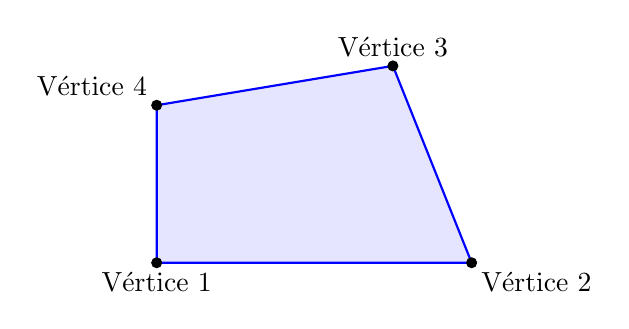
\begin{tikzpicture}
		% Desenho do polígono no plano
		\fill[blue!10] (0,0) -- (4,0) -- (3,2.5) -- (0,2) -- cycle;
		
		% Linhas (hiperplanos no plano)
		%\draw[thick, red] (0,2) -- (4,1.5) node[anchor=south east] {Hiperplano 1};
		%\draw[thick, green!70!black] (0,0) -- (4,3) node[anchor=south] {Hiperplano 2};
		%\draw[thick, purple] (0,3.5) -- (4,-0.5) node[anchor=north] {Hiperplano 3};
		
		% Polígono (interseção das restrições)
		\draw[thick, blue] (0,0) -- (4,0) -- (3,2.5) -- (0,2) -- cycle;
		
		% Vértices
		\fill[black] (0,0) circle (2pt) node[anchor=north] {Vértice 1};
		\fill[black] (4,0) circle (2pt) node[anchor=north west] {Vértice 2};
		\fill[black] (3,2.5) circle (2pt) node[anchor=south] {Vértice 3};
		\fill[black] (0,2) circle (2pt) node[anchor=south east] {Vértice 4};
		
		%Título
		%\node[below] at (2,-1) {\textbf{Figura 1: Interseção de hiperplanos em $\mathbb{R}^2$ (polígono)}};

	\end{tikzpicture}
	\caption{Interseção de hiperplanos em \(\mathbb{R}^2\)}
	\end{figure}
	
	%\vspace{2cm}
	\item No espaço tridimensional ($\mathbb{R}^3$): Um vértice de um poliedro é o ponto de encontro de três faces, que correspondem a hiperplanos em um espaço tridimensional.
	
	% Figura no espaço tridimensional (R^3)
	\begin{figure}[H]
	\centering
	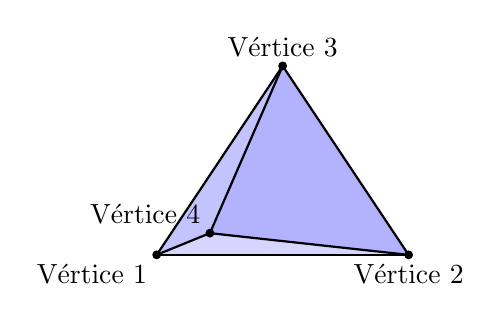
\begin{tikzpicture}[scale=0.8]
		% Poliedro (um tetraedro simples)
		\fill[blue!10,opacity=0.7] (0,0,0) -- (4,0,0) -- (2,3,0) -- cycle; % Base
		\fill[blue!20,opacity=0.7] (0,0,0) -- (4,0,0) -- (2,1.5,3) -- cycle; % Face lateral 1
		\fill[blue!30,opacity=0.7] (0,0,0) -- (2,3,0) -- (2,1.5,3) -- cycle; % Face lateral 2
		\fill[blue!40,opacity=0.7] (4,0,0) -- (2,3,0) -- (2,1.5,3) -- cycle; % Face lateral 3
		
		% Arestas do poliedro
		\draw[thick, black] (0,0,0) -- (4,0,0);
		\draw[thick, black] (4,0,0) -- (2,3,0);
		\draw[thick, black] (2,3,0) -- (0,0,0);
		\draw[thick, black] (0,0,0) -- (2,1.5,3);
		\draw[thick, black] (4,0,0) -- (2,1.5,3);
		\draw[thick, black] (2,3,0) -- (2,1.5,3);
		
		% Vértices
		\fill[black] (0,0,0) circle (2pt) node[anchor=north east] {Vértice 1};
		\fill[black] (4,0,0) circle (2pt) node[anchor=north] {Vértice 2};
		\fill[black] (2,3,0) circle (2pt) node[anchor=south] {Vértice 3};
		\fill[black] (2,1.5,3) circle (2pt) node[anchor=south east] {Vértice 4};
		
		% Título
		%\node[below] at (2,-1,0) {\textbf{Figura 2: Interseção de hiperplanos em $\mathbb{R}^3$ (poliedro)}};
	\end{tikzpicture}
	\caption{Interseção de Hiperplanos em $\mathbb{R}^3$}
	\end{figure}
\end{itemize}

Portanto, o conceito algébrico de ponto extremo está diretamente relacionado ao conceito geométrico de vértice. Concluímos que os pontos extremos de um conjunto viável de um PPL são, geometricamente, os vértices do poliedro formado por esse conjunto.
     

Pontos extremos desempenham um papel importante na Programação Linear, pois como veremos adiante, a solução ótima de um PPL sempre está em um ponto extremo do conjunto viável. Para o método simplex, a existência de pontos extremos degenerados requer precauções, pois esses podem afetar o desempenho do método, inclusive fazendo rodar indefinitivamente.   

\subsection{Raios e Direções}

Um raio também é uma classe de conjuntos convexos, que são definidos a seguir.

\begin{def:raio}
	Um raio $r$ é uma coleção de pontos dados na forma
	\begin{equation*}
		r = \{\mathbf{x} \in \mathbb{R}^n \ |\  \mathbf{x} + \lambda \mathbf{d}, \lambda > 0\}
	\end{equation*}
	onde $\mathbf{d}$ é um vetor em $\mathbb{R}^n$ não nulo e $\lambda$ é um real positivo
\end{def:raio}

Podemos também interpretar raios geometricamente como sendo uma semirreta com origem em $\mathbf{x}$, dito como o vértice do raio, e que se estende na direção do vetor $\mathbf{d}$, chamado de diretor ou direção do raio.

\begin{def:direção}
	Seja $X$ um conjunto convexo contido no $\mathbb{R}^n$. O vetor não nulo $\vec{d} \in \mathbb{R}^n$ é uma direção de $X$ com vértice em $\vec{x_0} \in X$ se para qualquer $\lambda \geq 0$ é verdade que $\vec{x_0} + \lambda \vec{d} \in X$  
\end{def:direção}

A Definição expande a noção de direção para qualquer conjunto convexo além dos raios. Dessa forma, uma direção pode ser entendida como uma semirreta que está contida num conjunto convexo. Disso segue que um conjunto convexo que possui uma direção não pode ser limitado, já que semirretas estendem-se indefinitivamente.

\begin{def:direção extrema}
	Seja $X$ um conjunto convexo e $\vec{d}$ uma direção desse conjunto. O vetor $\vec{d}$ é chamado de direção extrema se ele não pode ser dado como combinação linear positiva de outras direções desse conjunto.
\end{def:direção extrema}

A ideia de direções extremas é análoga a de pontos extremos. O vetor $\vec{d}$ é direção extrema se não existe outras duas direções $\vec{d}_1$ e $\vec{d}_2$ tal que
\begin{gather*}
	\lambda_1\vec{d}_1 + \lambda_2\vec{d}_2 = \vec{d} \\
	\lambda_1, \lambda_2 \geq 0
\end{gather*}
Os raios cuja a direção é dada por uma direção extrema são chamados de raios extremos.

Os conceitos de raios e direções podem ser usados para definir os cones convexos. Seja $C \subset \mathbb{R}^n$ um cone definido como \[C = \{\vec{x}\ |\ \lambda\vec{x}, \lambda \geq 0\}\]Podemos perceber que o subconjunto de $C$ dado pelos múltiplos escalares positivos de $\vec{x} \in C$ formam um raio com vértice na origem do $\mathbb{R}^n$ com direção dada por $\vec{x}$. Dessa forma, um cone pode ser definido a partir de suas direções, mas nem todas são necessárias para tal, já que podemos usar somente as suas direções extremas, que formam um conjunto minimal gerador das demais.

Portanto, se $C$ é um cone e $D = \{\vec{d}_1, \vec{d}_2, \ldots, \vec{d}_n\}$ o conjunto das suas direções extremas, então o cone pode ser dado como
\begin{equation*}
	C = \{\vec{x}\ |\ \vec{x} = \displaystyle\sum_{j = 1}^{n}
			\lambda_j \vec{d}_j, \lambda_j \geq 0\}
\end{equation*}

\begin{figure}[H]
\centering
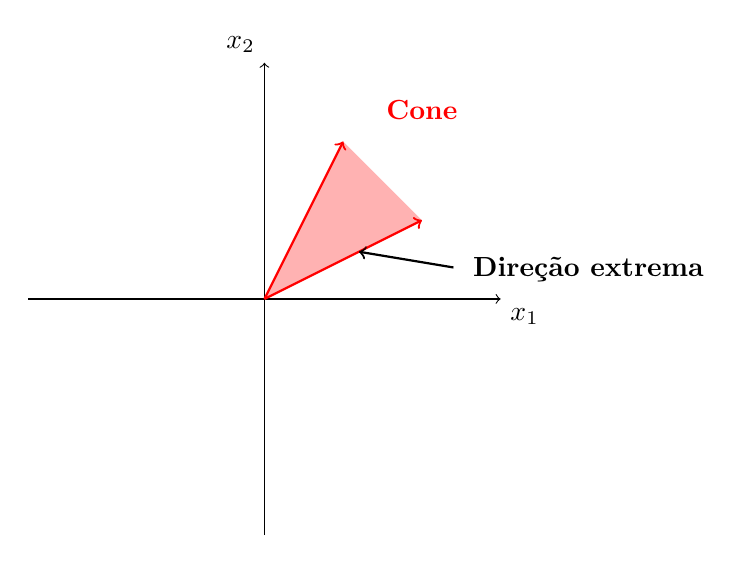
\begin{tikzpicture}[scale=2]
	
	% Eixos coordenados
	\draw[->] (-1.5, 0) -- (1.5, 0) node[below right] {\(x_1\)};
	\draw[->] (0, -1.5) -- (0, 1.5) node[above left] {\(x_2\)};
	
	% Semirretas (vetores que formam o cone)
	\draw[thick, red, ->] (0, 0) -- (1, 0.5) node[midway, above right] {};
	\draw[thick, red, ->] (0, 0) -- (0.5, 1) node[midway, above right] {};
	
	% Anotação para a direção extrema
	\draw[->, thick] (1.2, 0.2) -- (0.6, 0.3) node[pos=-0.1, right] {\textbf{Direção extrema}};
	
	
	% Região do cone (preenchida)
	\fill[red, opacity=0.3] (0, 0) -- (1, 0.5) -- (0.5, 1) -- cycle;
	
	% Vetores dentro do cone (exemplo de combinações convexas)
	%\draw[thick, blue, ->] (0, 0) -- (0.8, 0.6) node[midway, above] {};
	%\draw[thick, blue, ->] (0, 0) -- (0.4, 0.4) node[midway, above] {};
	
	% Adicionando um label para o cone
	\node[red] at (1, 1.2) {\textbf{Cone}};
\end{tikzpicture}
\caption{Representação de um Cone e seus raios extremos em \(\mathbb{R}^2\)}

\label{fig:cone}
\end{figure}

\subsection{Faces e Arestas}

Nesta seção apenas abordaremos algumas definições algébricas para conceitos historicamente geométricos. A primeira delas será a \textbf{face}.

\begin{def:face}
	Seja $X$ um conjunto convexo e $F = \{\vec{x} \in X\ |\ B\vec{x} = \vec{c}\}$ em que $B\vec{x} = \vec{c}$ é o sistema linear cujas equações é um subconjunto não vazio dos hiperplanos definidores de $X$. O conjunto $F$ é então chamado de face de $X$. 
\end{def:face}

Em outras palavras uma face é um subconjunto de $X$ cujos elementos são solução de um sistema linear dado por 1 ou mais hiperplanos de $X$. Em dimensão três, quando pensamos em faces de um poliedro, pensamos naquelas que tem dimensão dois, mas a nossa definição permite que outros elementos de dimensão menores, como as arestas e os vértices desse poliedro também sejam chamados de ``faces''. 

Na verdade, em dimensão $n$ podemos ter faces de qualquer dimensão entre 1 e $n$. As faces de dimensão $n - 1$, como as faces propriamente ditas de um poliedro em dimensão 3, ou as arestas de um polígono bidimensional, são chamadas de \textbf{facetas}. Facetas também podem ser entendidas como a parte viável (que está em $X$) de um hiperplano definidor.  As faces com dimensão entre $n - 1$ e $0$ são chamadas de faces próprias de $X$, enquanto aquela de dimensão $n$, que é o próprio $X$ é chamada de face imprópria\footnote{Se nossa definição considerasse o conjunto vazio também como face de um conjunto convexo, então ele também seria uma face imprópria}.

Vamos agora dizer que $r(F)$ da face $F$ de um conjunto convexo $X$ é o número mínimo de hiperplanos necessários para definir $F$ como o conjunto solução de um sistema linear. Esse número, para pontos extremos, que são faces de dimensão 0, é $n$, como vimos no teorema \ref{thm:ponto extremo}. Para uma aresta, que é um segmento de reta, e possui, pois, dimensão 1, esse número é $n - 1$. Podemos concluir que no geral a dimensão $\dim(F)$ de uma face $F$ e o número $r(F)$ estão relacionadas por
\begin{equation*}
	r(F)= n - \dim(F)
\end{equation*} 

Ainda sobre arestas, sabemos da geometria clássica que elas sempre conectam dois vértices, par esse chamado de adjacentes. Como vimos, pontos extremos equivalem aos vértices de um poliedro convexo $n$ dimensional, e, analogamente, os pontos extremos que são conectados por uma aresta (o que nem sempre ocorre, visto que os poliedros podem ser ilimitados) são também chamados de \textbf{adjacentes}. A Proposição a seguir mostra que dois vértices produzem uma aresta.

\begin{prop:aresta}
	O conjunto das combinações convexas de dois pontos extremos de um conjunto convexo $X$ é uma aresta de $X$
	
	\begin{proof}
		Sejam $\vec{x}_1$ e $\vec{x}_2$ pontos extremos de $X$, e digamos que $R$ e $S$ sejam os conjunto dos hiperplanos definidores de $X$ aos quais $\vec{x}_1$ e $\vec{x}_2$ pertencem respectivamente. Sob a hipótese de que $\vec{x}_1$ e $\vec{x}_2$ são distintos, então $R \cap S$ possui $n - 1$ hiperplanos, que por sua vez, devem se intersectar em uma face $E$ de dimensão $1$.
		
		Seja $C$ é o conjunto das combinações lineares convexas de $\vec{x}_1$ e $\vec{x}_2$, iremos provar que $C = E$. Primeiramente, temos que $E$ é um conjunto convexo por ser a interseção de conjuntos convexos, e como $\vec{x}_1$ e $\vec{x}_2$ pertencem a $E$, então suas combinações convexas, dadas por $C$, devem estar contidas em $E$.
		
		O próximo passo é mostrar que todos os pontos de $E$ são combinações convexas de $\vec{x}_1$ e $\vec{x}_2$, e usaremos um argumento geométrico para isso. O conjunto $E$ está numa reta, pois tem dimensão $1$, e da geometria básica sabemos que uma reta é definida por no mínimo dois pontos. Se existisse um ponto $\vec{x}_3 \in E$ que não é combinação convexa de $\vec{x}_1$ e $\vec{x}_2$, então $\vec{x}_3$ não pode estar entre $\vec{x}_1$ e $\vec{x}_2$, o que nos leva a dois casos
		\begin{itemize}
			\item $\vec{x}_1$ está entre $\vec{x}_3$ e $\vec{x}_2$
			
			\item $\vec{x}_2$ está entre $\vec{x}_1$ e $\vec{x}_3$
		\end{itemize}
		Os dois casos levam a um absurdo, pois ou $\vec{x}_1$ ou $\vec{x}_2$ estaria entre dois pontos de $E$ e não seria um ponto extremo. Concluímos então que $C = E$, e as combinações convexas de dois vértices é uma aresta. 
	\end{proof}
\end{prop:aresta}

Repare que a recíproca da proposição não é verdadeira, e um exemplo simples é o cone, como mostrado na figura \ref{fig:cone}, que possui apenas um vértice na origem, e duas arestas que se prolongam indefinitivamente. 

A ideia de adjacência entre vértices é bem simples, mas é aplicada no método simplex. Como citamos anteriormente, a busca das soluções ótimas de um PPL pelo simplex se dá nos pontos extremos da região viável, e a forma como ele realiza essas buscas é percorrendo as arestas do conjunto, ou seja, ele parte de um ponto extremo e segue a busca em um ponto extremo adjacente sempre.  


% -------------------------- DEFINIÇÃO --------------------
\newtheorem{def:convex hull}[def:conjunto convexo]{Definição}
\newtheorem{def:independencia convexa}[def:conjunto convexo]{Definição}
\newtheorem{def:simplex}[def:conjunto convexo]{Definição}
\newtheorem{def:combinação afim}[def:conjunto convexo]{Definição}

% ------------------------- PROPOSIÇÃO --------------------
\newtheorem{prop:redundancia}[prop:combinação convexa]{Proposição}
\newtheorem{prop:pontos extremos na fronteira}[prop:combinação convexa]{Proposição}
\newtheorem{prop:conjuntos convexos fechados}[prop:combinação convexa]{Proposição}
\newtheorem{prop:conjuntos convexos limitados}[prop:combinação convexa]{Proposição}

% ------------------------------ LEMA --------------------------
\newtheorem{lemma:afim}{Lema}[chapter]

%------------------------------ TEOREMA ---------------------------
\newtheorem{thm:caratheodory}{Teorema}[chapter]
\newtheorem{thm:conjuntos convexos compactos}[thm:caratheodory]{Teorema}

% ---------------------------- COROLÁRIO -----------------------
\newtheorem{cor:caratheodory}{Corolário}[chapter]

\section{Geometria dos Poliedros Convexos}

Nesta seção iremos obsevar os poliedros convexos a partir de sua
natureza geométrica ao mesmo tempo que mostramos sua equivalência com
os conceitos algébricos vistos nas seções anteriores.

\subsection{Envoltória Convexa}

\begin{def:convex hull}
	\label{def:convex hull}
	Seja $P$ um conjunto de pontos em $\mathbb{R}^n$. Chamamos de envoltória
	convexa $P$, ou fecho convexo, o conjunto
	$\conv{P}$ dado por todas as combinações convexas dos pontos de $P$
\end{def:convex hull}

Em outras referências, pode-se encontrar uma definição equivalente de que a
envoltória convexa, também popularmente conhecida como \textit{covex hull},
é o menor conjunto convexo que contém todos os pontos de $P$. Neste texto,
usaremos a definição destacada por ela ser mais algebricamente fecunda.

\begin{def:independencia convexa}
	Seja $P \subset \mathbb{R}^n$ é um conjunto de pontos. $P$ é convexo-independente
	se nenhum de seus pontos pode ser dado como combinação convexa de outros dois.
\end{def:independencia convexa}

A definição acima especializa o conceito de independência linear para conjuntos convexos,
que nos será uma definição útil. Dessa forma, um conjunto convexo-dependente será aquele
no qual há pelo menos um ponto que pode ser dado como combinação convexa de outros dois.
Outra especialização que faremos será do conceito de geradores: se um conjunto convexo
$X$ é a envoltória convexa de um conjunto $P$, então $P$ é um conjunto gerador de $X$.
Ademais, se $P$ é convexo-independente, então os pontos de $P$ são os pontos extremos
de $X$, o que especializa o conceito de base da álgebra linear para os pontos extremos.

Na Teoria de PL, nosso interesse irá se concentrar nos conjuntos convexo que são
finitamente gerados, isto é, que podem ser determinados por um conjunto finito
de pontos geradores. Exemplo de conjuntos convexos finitamente gerados são
os poliedros tridimensionais e os polígonos, enquanto que o círculo, ou a esfera,
são exemplos de conjuntos convexos que não são finitamente gerados.

\begin{figure}[h]
\centering
% Primeira figura: Polígono Convexo
\begin{subfigure}{0.45\textwidth}
	\centering
	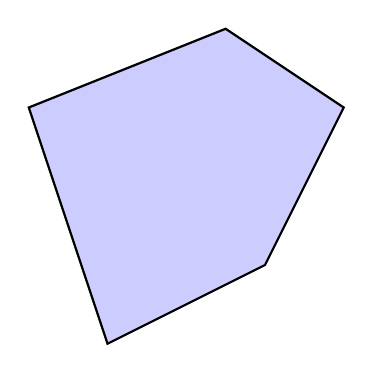
\begin{tikzpicture}
		\draw[thick, fill=blue!20] (0,0) -- (2,1) -- (3,3) -- (1.5,4) -- (-1,3) -- cycle;
	\end{tikzpicture}
	\caption{Conjunto convexo finitamente gerado}
	\label{fig:poligono}
\end{subfigure}
\hfill
% Segunda figura: Círculo
\begin{subfigure}{0.50\textwidth}
	\centering
	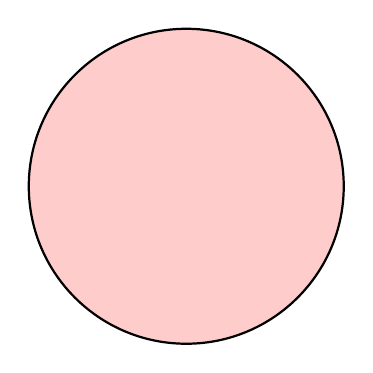
\begin{tikzpicture}
		\draw[thick, fill=red!20] (0,0) circle (2);
	\end{tikzpicture}
	\caption{Conjunto convexo não finitamente gerado}
	\label{fig:circulo}
\end{subfigure}
\caption{Comparação entre um polígono convexo e um círculo.}
\end{figure}

\begin{prop:redundancia}
	Seja $P = \{p_1, \ldots, p_m\}$ um conjunto convexo dependente e
	$P' = \{p_1, \ldots, p_k\}$ um subconjunto convexo-independente
	de $P$ com $k < m$. Então é correto dizer que
	\begin{equation*}
		\conv{P'} = \conv{P}
	\end{equation*}
\end{prop:redundancia}

Dado um conjunto de geradores, é fácil observar que, ao obtermos um
novo conjunto sem as redundâncias, então a envoltória convexa, como
foi definida em \ref{def:convex hull}, será exatamente a mesmas para
ambos os conjuntos. Além disso, se $P$ for um conjunto convexo
independente, então seus elementos são os pontos extremos de \(\conv{P}\),
como fora observado mais previamente.

Uma classe especial de envoltórias convexas são os \textbf{simplex}
A ideia geométrica por detrás do conceito de simplex é do ``mais simples
conjunto convexo num espaço euclideano de dimensão finita''. Por exemplo:
o menor número de pontos necessários para delimitar uma região no plano é
3, e a região delimitada por eles é um triângulo. Já em dimensão 3, para
delimitar uma região no espaço são necessários ao menos quatro pontos,
que definirão um tetraedro. Generalizando essa primitiva, obtemos a definição.

\begin{def:simplex}
	Chama-se simplex a envoltória convexa de um conjunto de $n+1$ pontos
	em $\mathbb{R}^n$ convexo-independente.
\end{def:simplex}

\begin{figure}[h]
	\centering
	% Primeira figura: Triângulo
	\begin{subfigure}{0.45\textwidth}
		\centering
		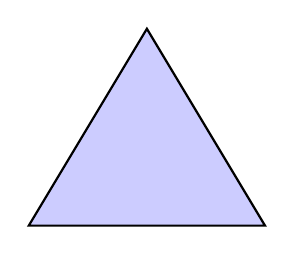
\begin{tikzpicture}
			\draw[thick, fill=blue!20] (0,0) -- (3,0) -- (1.5,2.5) -- cycle;
		\end{tikzpicture}
		\caption{Simplex em 2D}
		\label{fig:triangulo}
	\end{subfigure}
	\hfill
	% Segunda figura: Tetraedro em 3D
	\begin{subfigure}{0.45\textwidth}
		\centering
		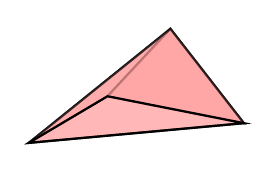
\begin{tikzpicture}
			% Definição dos vértices
			\tdplotsetmaincoords{70}{120}
			\begin{scope}[tdplot_main_coords]
				% Arestas do tetraedro
				\draw[thick, fill=red!20, opacity=0.7] (0,0,0) -- (2,0,0) -- (1,1.5,1.5) -- cycle;
				\draw[thick, fill=red!30, opacity=0.7] (0,0,0) -- (1,1.5,1.5) -- (0,2,0) -- cycle;
				\draw[thick, fill=red!40, opacity=0.7] (2,0,0) -- (1,1.5,1.5) -- (0,2,0) -- cycle;
				\draw[thick] (0,0,0) -- (2,0,0) -- (0,2,0) -- cycle;
			\end{scope}
		\end{tikzpicture}
		\caption{Simplex em 3D}
		\label{fig:tetraedro}
	\end{subfigure}
	\caption{Comparação entre simplex de dimensões diferentes.}
\end{figure}

\subsection{Espaços Afim}

Antes de ir mais afundo na natureza geométrica dos conjuntos
poliédricos, iremos recuar um pouco e observar alguns conceitos
algébricos. Relembrando, uma das noções primárias da Álgebra Linear é a de
independência linear, em que dizemos que um conjunto de vetores
é linearmente independente se nenhum vetor poder ser dado
como combinação linear dos demais. Uma classe de combinações
lineares que nos é últil são as chamadas combinações afim

\begin{def:combinação afim}
Sejam $v_1, \ldots, v_k$ vetores do $\mathbb{R}$. $u$ é uma
combinação afim dos vetores citados  se existem $\lambda_1, \ldots,
\lambda_k$ tal que
\begin{equation*}
	u = \sum_{i =1}^{k}\lambda_i v_i \quad \quad \sum_{i=1}^{k} \lambda_i = 1
\end{equation*}
\end{def:combinação afim}
Combinações afim são uma especialização das combinações
lineares, visto a restrição de que a soma dos escalares
que acompanham os vetores deve ser igual a 1. Observemos
também que as combinaçãoes convexas, por sua vez, são uma
especialização das combinações afim, em que adiciona-se a
restrição de que os pesos devem ser positivos.

As combinações lineares afim de um conjunto de vetores
formam um conjunto fechado chamado de \textbf{subsespaço afim},
que são análogos aos hiperplanos lineares a menos
da restrição de conterem a
origem do $\mathbb{R}^n$.

% imagem de compração de um hiperplano linear
% e um afim

Os hiperplanos  afins, de forma análoga ao lineares, podem ser
definidos a partir de um sistema linear na forma $Ax = b$
ou através de um conjunto de no mínimo $n$ geradores.
Um conjunto de vetores em que pelo menos um dos membros
é combinação afim dos demais é chamado de afimmente dependente.
Geometricamente, isso significa que pelo menos um dos vetores estará
no espaço afim gerado pelos demais.

É sabido que qualquer conjunto com mais de $n$ vetores em
$\mathbb{R}^n$ é linearmente dependente, mas qual será o número mínimo
de vetores em um conjunto para afirmamos com certeza que eles são
afimmente dependentes?

A envoltória convexa de dois pontos é um segmento de reta, e,
por sua vez, o subsespaço afim gerado por esses mesmos pontos é a
a própria reta que eles definem, ou seja, obtemos o subespaço
afim gerado ao extender infinitamente o segmento de reta em
ambos os seus sentido. Já três pontos não colineares
definem um triângulo, que é uma figura plana, e o subsespaço afim gerado por
esses três pontos é justamnte o plano que contém esse triângulo; é como se
tivessemos expandido infinitamente a área do triângulo assim como fizemos
com o comprimento do segmento de reta anteriormente. Por conseguinte,
para obter o \textit{span} afim a partir de uma envoltória convexa, basta
extendemos infinitamente a envoltória nas direções possíveis.

Isso nos permite agora responder a questão feita mais atrás:
expandir infinitamente um simplex de dimensão $n$ que é gerado
por $n+1$ vetores do  $\mathbb{R}^n$,
, é suficiente para obtermos todo o $\mathbb{R}^n$
e qualquer outro vetor do $\mathbb{R}^n$ pode ser dado como
combinação afim dos pontos extremos do simplex que fora expandido.
Portanto, a conclusão que chegamos é que qualquer conjunto com mais
de $n+1$ vetores é necessariamnte afimmente independente. Esse resultado
é provado formalmente com uma abordagem mais algébrica no lema a seguir.

\begin{lemma:afim}
	\label{lemma:afim}
	Se $P = \{p_1, \ldots, p_k\} \subset \mathbb{R}^n$ é um conjunto
	finito de pontos com $k > n + 1$, então existem $\mu_1, \ldots, \mu_n
	\in \mathbb{R}$ não todos nulos tal que
	\begin{equation*}
		\displaystyle\sum_{i=1}^k \mu_i p_i = 0 \quad\quad \displaystyle\sum_{i=1}^k \mu_i = 0
	\end{equation*}
	e $P$ é um conjunto afimmente dependente.

	\begin{proof}
		Da álgebra linear, sabemos que, se $\#P = k > n$, então $P$ é um conjunto
		linearmente dependente, o que implica dizer que há $\mu_1, \ldots, \mu_n
		\in \mathbb{R}$ não todos nulos tal que
		\[\displaystyle\sum_{i=1}^k \mu_i p_i = 0\]

		Além disso, observemos que o conjunto $\{p_2 - p_1, \ldots, p_k - p_1\}$
		também é linearmente dependente, portanto
		\[\displaystyle\sum_{i=2}^k \mu_i (p_i - p_1) = 0\]
		e fazendo \(\mu_1 = -\displaystyle\sum_{i=2}^k \mu_i\)
		obtemos que
		\[\displaystyle\sum_{i=1}^k \mu_i = 0\]

		Resta mostrar que o conjunto $P$ é afimmente dependente. Para isso, suponha
		que $P$ esteja ordenado de forma que para todo $i \in I = \{1, \ldots, n\}$
		é verdade que $\mu_k \geq \mu_i$. Obeservamos então que
	  \begin{gather*}
	    \mu_1 p_1 + \ldots + \mu_{k - 1} p_{k-1} + \mu_k p_k = 0 \\
      \mu_1 p_1 + \ldots + \mu_{k - 1} p_{k-1} = - \mu_k p_k \\
	  \end{gather*}
	  Dividindo a equação acima toda por $-\mu_k$ otbemos
	  \begin{gather*}
	    \sum_{i=1}^{k-1} -\frac{\mu_i}{\mu_k} p_i = p_k
	  \end{gather*}
	  Mas também
	  \begin{gather*}
      \sum_{i=1}^{k-1} \mu_i = 0 \\
	    \sum_{i=1}^{k-1} -\frac{\mu_i}{\mu_k} = 1
	  \end{gather*}
	  Portanto $p_k$ pode ser dado como combinação afim dos demais pontos de
	  $P$, e o conjunto dos pontos é afimmente dependente.
	\end{proof}
\end{lemma:afim}

\subsection{Teorema de Carathéodory}

O Teorema de Carathéodory é um dos resultados mais fundamentais da geometria
convexa, pois ele nos permite dizer que um ponto qualquer em um conjunto
convexo pode ser gerado por um número finito de outros pontos nesse conjunto,
mas não somente isso como também o limitante do tamanho desse conjunto de
geradores.

\begin{thm:caratheodory}[Carathéodory]
	Seja $P \subset \mathbb{R}^n$ um conjunto finito de pontos. Se $x \in \conv{P}$, então
	$x \in \conv{P'}$ para algum $P' \subset P$ com cardinalidade igual a $n + 1$.

	\begin{proof}
		Com efeito, se $x \in \conv{P}$, e $\#P = k$, então existem $\lambda_1, \ldots, \lambda_k
		\in \mathbb{R}$ com $\lambda_i \in [0, 1]$ tal que
		\begin{equation}
		\label{eq_thm_caratheory}
		\begin{gathered}
			x = \displaystyle\sum_{i=1}^k \lambda_i p_i \\
			\displaystyle\sum_{i=1}^k \mu_i = 1
		\end{gathered}
		\end{equation}
		Se $k \leq n + 1$, então nada há a demonstrar, do contrário, o lema \ref{lemma:afim}
		garante que existem $\mu_1, \ldots, \mu_n \in \mathbb{R}$ não todos nulos tal que
		\[\displaystyle\sum_{i=1}^k \mu_i p_i = 0\]
		e como \(\alpha \displaystyle\sum_{i=1}^k \mu_i p_i = 0\) para todo $\alpha \in \mathbb{R}$
		então podemos rescrever a equação \ref{eq_thm_caratheory} como
		\begin{gather*}
			x = \displaystyle\sum_{i=1}^k \lambda_i p_i - \alpha \displaystyle\sum_{i=1}^k \mu_i p_i \\
			x = \displaystyle\sum_{i=1}^k (\lambda_i - \alpha \mu_i) p_i
		\end{gather*}
		donde temos que
		\[\displaystyle\sum_{i=1}^k (\lambda_i - \alpha \mu_i) = 1\]

		Agora iremos tentar escrever $x$ como uma combinação convexa de até $n + 1$ pontos.
		Para atingir esse objetivo, escolhemos $\alpha$ tal que
	\[\alpha  = \min{\frac{\lambda_i}{\mu_i}\  |\  i \in \{1,\ldots, k\} \text{ e } \mu_i > 0}\]
		Logo, $\alpha > 0$, e para $i \in \{1, \ldots, k\}$, temos dois casos.

		I - $\mu_i \geq 0$

		Temos que
		\[\lambda_i - \alpha \mu_i = \mu_i \left(\frac{\lambda_i}{\mu_i} - \alpha\right)\]
		e pela nossa escolha de $\alpha$, então \(\lambda_i - \alpha \mu_i \geq 0\)

		II - $\mu_i < 0$

		Uma vez que $\alpha > 0$, então $\alpha \mu_i > 0$ e, portanto,
		\(\lambda_i - \alpha \mu_i \geq 0\)

		digamos que $j*$ seja tal que $\alpha = \frac{\lambda_{j^*}}{\mu_{j^*}}$. Observe que
		$\lambda_{j^*} - \alpha \mu_{j^*}$, e podemos expressar $x$ como
		\[x = \displaystyle\sum_{i=1}^{j^* - 1} (\lambda_i - \alpha \mu_i)p_i +
				\displaystyle\sum_{i=j^* + 1}^{k} (\lambda_i - \alpha \mu_i)p_i\]
		donde concluímos que $x$ pode ser escrito como combinação convexa de $k - 1$ pontos de $conv{P}$

		Como podemos repetir esse processo enquanto $k > n + 1$, ou seja, enquanto o lema \ref{lemma:afim}
		pode ser aplicado, então $x$ pode ser escrito como combinação convexa de até $n + 1$ pontos de $\conv{P}$.
	\end{proof}
\end{thm:caratheodory}

Para capturar o significado geométrico do Teorema de Carathéodory, poderíamos
enunciá-lo como ``um ponto qualquer num fecho convexo sempre estará no interior
de um simplex gerado por pontos desse fecho''. Ademais, se $P \subset \mathbb{R}^n$ é um conjunto
convexo-independente, então para qualquer $x \in \conv{P}$, $x$ pode ser dado
como combinação convexa de até $n+1$ pontos de $P$, ou seja, de até $n+1$ pontos extremos.
Formalizemos essa conclusão como corolário do Teorema de Carathéodory.

\begin{cor:caratheodory}
	Seja $P \subset \mathbb{R}^n$ um conjunto convexo-independente. Se $x \in \conv{P}$
	então $x$ pode ser dado como combinação convexa de até $n + 1$ pontos de $P$
\end{cor:caratheodory}

Em outras palavras, o corolário afirma que um ponto qualquer num fecho convexo
pode ser dado como combinação convexa de até $n+1$ pontos extremos.

\subsection{Topologia de Evoltórias Convexas}

Nesta seção iremos analisar algumas propriedades topológicas básicas de
interesse sobre a envoltória convexa de um conjunto de pontos. Mas não se
preocupe, apesar de usarmos conceitos de topologia, iremos apresentá-los
e usá-los de forma bem elementar a fim de não desviar muito dos nossos
objetios e complicar em demasiado nossas construções, já que está fora do
escopo desse texto as noções mais aprofundadas desse tema.

\begin{prop:pontos extremos na fronteira}
Seja $P$ um conjunto convexo. Se $\bar{\vec{x}}$ é um ponto extremo de $P$,
então $\bar{\vec{x}}$ é um ponto na fronteira de $P$.

  \begin{proof}
    Para provarmos esse resultado, basta mostrarmos que para qualquer bola
    aberta $B$ centrada em $\bar{\vec{x}}$, $B$ intercepta pontos tanto de
    $P$ quanto de $\mathbb{R}^n / P$. Suponha por contradição que haja uma
    bola aberta centrada em $\bar{\vec{x}}$ tal que $B \subsetneq P$. Isso
    implica que $\bar{\vec{x}}$ está no interior de um segmento de reta
    inteiramente contido em $P$, e não é, pois, ponto extremo.
  \end{proof}
\end{prop:pontos extremos na fronteira}

\begin{prop:conjuntos convexos fechados}
Se $C$ é a envoltória convexa de $P$, então $C$ é fechado.

  \begin{proof}
   Seja $\vec{x}$ um ponto na fronteira $F$ de $C$. É trivial o fato de que se
   $\vec{x}$ é um ponto extremo de $C$, então $\vec{x} \in P$. Se
   $\vec{x} \in F$ não for um ponto extremo, então uma vez que $\vec{x} \in F$,
   temos que existe uma vizinhança $V$ de $\vec{x}$ que contém um ponto $\vec{y}$
   tal que $\vec{y} \in C$.

   Digamos que $\vec{d} = \vec{x} - \vec{y}$, e todo ponto dado como \[
     \vec{y} + (1 - \epsilon) \vec{d}
   \]com $\epsilon \in (0, 1]$ faz parte de um raio contido em $C$. Repare que
   esse ponto é $x$ quando $\epsilon = 0$. Digamos também que \[
     \vec{y} = \sum_{i=1}^{k} \lambda_i \vec{p_i}, \quad \vec{p_i}  \in P
   \]Das equações dadas até então, temos que
   \begin{align*}
     \vec{y} + (1 - \epsilon) (\vec{x} - \vec{y}) &= (1 + \epsilon) \vec{x}
     + \epsilon y \\
                                                  &= (1 - \epsilon) \vec{x} + \epsilon \vec{y}
   \end{align*}
   Reparemos que como estamos considerando os pontos do raio que estão no
   interior de $C$, então esses pontos
   admitem uma representação como uma combinação linear convexa dos pontos de
   $P$, ou seja
   \[
     \forall \epsilon \in (0, 1] , \exists \mu_1, \dots, \mu_k \in \mathbb{R},
     (1-\epsilon)\vec{x} + \epsilon \vec{y} = \sum_{i=1}^{k} \mu_i p_i
   \]
   Isolando $\vec{x}$ na equação acima, e adotando a representação de $\vec{y}$
   como combinação convexa, obtemos que

   \begin{equation}
     \label{eq:conjunto convexos fechados}
     \vec{x} = \sum_{i=1}^{k} \frac{(\mu_i  - \epsilon \lambda)}{1-\epsilon} \vec{p_i}
   \end{equation}
   Percebamos que
   \[
    \sum_{i=1}^{k} \frac{(\mu_i  - \epsilon \lambda)}{1-\epsilon} =
    \frac{1}{1-\epsilon}\left(
      \sum_{i=1}^{k} \mu_i -   \epsilon \sum_{i=1}^{k} \lambda_i\right)
   \]
   Uma vez que
   \[
    \sum_{i=1}^{k} \mu_i = 1 \quad \sum_{i=1}^{k} \lambda_i = 1
   \]
   obtém-se que
   \[
   \sum_{i=1}^{k} \frac{(\mu_i  - \epsilon \lambda)}{1-\epsilon} =
   \frac{1}{1-\epsilon} \cdot (1 - \epsilon) = 1
   \]
   o que vale para todo $\epsilon \in [0, 1]$.

   Se fazemos $\epsilon$ pequeno o suficiente, então a equação
   \ref{eq:conjunto convexos fechados} expressa $\vec{x}$ como combinação
   convexa de pontos de $P$
   \[
     \lim_{\epsilon \to 0} \sum_{i=1}^{k} \frac{(\mu_i  - \epsilon \lambda)}{1-\epsilon} \vec{p}_i
     = \sum_{i=1}^{k} \mu_i \vec{p}_i
   \]
   Portanto, se $\vec{x}$ está na fronteira de $C = \conv{P}$, então
   $\vec{x} \in C$.
 \end{proof}
\end{prop:conjuntos convexos fechados}

\begin{prop:conjuntos convexos limitados}
  Se $C = \conv{P}$ é a envoltória convexa de um conjunto finito $P$ de pontos,
  então $C$ é limitado.

  \begin{proof}
   Com efeito, uma vez que $P$ é finito, então deve have uma bola aberta que
   contém todos os seus pontos e, por conseguinte, a envoltória convexa desse
   conjunto, portanto $C = \conv{P}$ é limitado.
  \end{proof}
\end{prop:conjuntos convexos limitados}

Para fins de síntese, reunamos as proposiçõe anteriores no teorema a seguir

\begin{thm:conjuntos convexos compactos}
  Se $C = \conv{P}$ é a envoltória convexa de um conjunto finito de pontos,
  então $C$ é compacto.\footnote{Chama-se de compactos os conjuntos que são
  simultâneamente fechados e limitados.}
\end{thm:conjuntos convexos compactos}


\chapter{Teoria da Programação Linear}
% conjuntos convexos
% semiespaços e hiperplanos
% funções convexas
% direções extremas e conjuntos ilimitados
% fecho convexo
% cone convexo
% cone poliédrico
% polítopos e poliedros
% representação de conjuntos poliédricos

\theoremstyle{definition}

\newtheorem{def:conjunto convexo}{Definição}[chapter]

\newtheorem{def:politopo}[def:conjunto convexo]{Definição}

\newtheorem{def:poliedro convexo}[def:conjunto convexo]{Definição}

\newtheorem{def:cone}[def:conjunto convexo]{Definição}

\newtheorem{def:cone convexo}[def:conjunto convexo]{Definição}

\newtheorem{def:cpc}[def:conjunto convexo]{Definição}



\section{Espaços Convexos}

\subsection{Conjuntos Convexos}

Um dos conceitos mais fundamentais para a Teoria de PL é a de \textbf{convexidade}. Na Geometria, convexidade é definida como a propriedade de uma figura em que, para quaisquer pontos no seu interior, o segmento de reta entre esses pontos está inteiramente contido na figura. Mas podemos definir convexidade algebricamente da seguinte forma:

\begin{def:conjunto convexo}
	\label{def:conjunto convexo}
	Um conjunto $\mathbb{V}$ no $\mathbb{R}^n$ é chamado convexo se para quaisquer vetores $x_1, x_2 \in \mathbb{V}$ é verdade que \[\lambda x_1 + (1 - \lambda)x_2 \in \mathbb{V}\] para todo $\lambda \in [0, 1]$
\end{def:conjunto convexo}

Aqueles com algum conhecimento de geometria analítica devem se lembrar que uma combinação linear de vetores na forma $\lambda x_1 + (1 - \lambda)x_2$ com $\lambda \in [0, 1]$ define o segmento de reta que une as extremidades desses vetores. Esse tipo de combinação é chamada de convexa.

De forma mais geral, uma combinação linear convexa é aquela em que a soma dos escalares é igual a 1. Então supondo um conjunto de geradores formado por $x_1, \ldots, x_n$ e escalares $\lambda_1, \ldots, \lambda_n$, então a combinação linear
\[x = \sum_{i=1}^{n} \lambda_i x_i\] é convexa se \[\sum_{i=1}^{n} \lambda_i = 1\]



\subsection{Semiespaços e Hiperplanos}
Semiespaços e hiperplanos generalizam o conceito geométrico do plano que é dividido por um reta, gerando-se dois semiplanos. Um hiperplano no $\mathbb{R}^n$ é um espaço de dimensão $n-1$ que divide o primeiro em dois semiespaços. 

Algebricamente, um hiperplano $H$ é o conjunto dos vetores $x \in \mathbb{R}^n$ que solucionam uma equação linear na forma $a^\top x = k$, onde $k \in \mathbb{R}$ é uma constante e $a \in \mathbb{R}^n$ é um vetor não nulo, geralmente conhecido como vetor normal ou gradiente.

\begin{equation*}
	H = \{x\ |\ a^\intercal x = k\}
\end{equation*} 

Por sua vez, semiespaços são definidos algebricamente como inequações lineares. Se $H$ é um hiperplano no $\mathbb{R}^n$ definido pela equação $a^\intercal x = k$, então esse hiperplano divide o $\mathbb{R}^n$ em hiperespaços $H^+$ e $H^-$ que podem ser dados por
\begin{align*}
	H^+ = \{x \ |\ a^\intercal x  \geq k\} \quad
	H^- = \{x \ |\ a^\intercal x  \leq k\} 
\end{align*}
ou por
\begin{align*}
	H^+ = \{x \ |\ a^\intercal x  > k\} \quad
	H^- = \{x \ |\ a^\intercal x  < k\} 
\end{align*}

Os primeiros são \textbf{semiespaços fechados}, isto é, eles incluem sua fronteira, que consiste do hiperplano $H$. Por sua vez, os segundos são \textbf{semiespaços abertos}, pois não incluem sua fronteira. Tanto hiperplanos quanto semiespaços são conjuntos convexos. A demonstração disso fica como exercício para o leitor.

Caso se lembres da forma como expressamos as restrições de um PPL, perceberás que o conjunto viável é na verdade a interseção de vários semiespaços fechados. Portanto, se $R$ é a região factível do PPL cujo conjunto de restrições é dado por $Ax \leq b$, por exemplo, então 
\[R = \{x \ | \ Ax \leq b\}\]
e como a interseção de conjuntos convexos é também convexo, então as restrições de um problema de programação linear formam um conjunto convexo.

\subsection{Poliedros e Politopos}
Normalmente, aprendemos no ensino básico que poliedros são figuras tridimensionais formadas por faces poligonais. Por sua vez, polígonos seriam figuras bidimensionais limitadas, ou seja possuem uma área finita, formadas por segmentos de retas que se encontram em pontos chamados de vértices.

Politopos surgem como uma espécie generalização dos conceitos clássicos de polígonos e poliedros \textbf{convexos} para o caso n-dimensional. Dessa forma, poliedros convexos, por exemplo, seriam politopos tridimensionais, enquanto que os polígonos convexos são politopos bidimensionais. 

Apesar da noção clássica de poliedros se limitar ao caso tridimensional, a literatura matemática estende este conceito para n dimensões. Contudo, a definição formal de um poliedro de n-dimensões não é um consenso, e não é difícil encontrar definições diferentes, e por vezes não equivalentes, do que se trata esse objeto matemático.

Dito isso, e pelo fato da Teoria de PL se concentrar mais especificamente na classe dos poliedros \textbf{convexos}, que são melhores definidos, não iremos tratar das outras classes. Dessa forma, segue uma definição conveniente para ao Teoria de PL do que é um poliedro convexo.

\begin{def:poliedro convexo}
	Um poliedro convexo é a interseção de um número finito de semiespaços.
\end{def:poliedro convexo}

Por sua vez, politopos são dados como

\begin{def:politopo}
	Um politopo é um poliedro convexo limitado
\end{def:politopo}

Para aqueles que não lembrarem, o conceito de limitado na matemática não é equivalente ao de finito. Formalmente, um conjunto limitado é aquele que pode ser contido dentro de uma bola de raio finito. 

Das definições percebemos que poliedros convexos podem ser dados como um sistema de inequações ou equações lineares. Por conseguinte, o espaço das soluções viáveis $R$ de um problema de PL é um poliedro convexo. Contudo, nem sempre esse espaço será um politopo, pois nem sempre temos um conjunto limitado de soluções factíveis.

\subsection{Cone Convexo}

Algebricamente, um cone é definido como um conjunto $C$ em que para todo $\mathbf{x} \in C$ e todo $\lambda \in \mathbb{R}$ não negativo é verdade que \(\lambda \mathbf{x} \in C\). Dessa definição segue que a origem sempre é um membro do cone, caso em que $\lambda = 0$. Uma classe especial dos cones são os convexos, que são definidos como

\begin{def:cone convexo}
	Um cone $C$ é convexo se para quaisquer $\mathbf{x_1, x_2} \in C$ temos que $\mathbf{x_1} + \mathbf{x_2} \in C$
\end{def:cone convexo}

Do que foi dito até então, é fácil ver que, se a soma de quaisquer elementos de um cone está nele, então uma combinação linear convexa também estará.

Uma classe ainda mais especial dos cones, são os cones poliédricos convexos

\begin{def:cpc}
	Se $A$ é um matriz $m \times n$, então um cone poliédrico convexo $C$ é aquele definido por
	\begin{equation*}
		C = \{\vec{x}\ |\ A \vec{x} \leq 0\}
	\end{equation*}  
\end{def:cpc}

Uma propriedade interessante dessa classe de cones é que a iésima linha da matriz $A$ é o vetor normal ao íésimo semiespaço dado por \[\mathbf{a^\intercal x} \leq 0\]Os cones poliédricos convexos desempenham um importante papel na Teoria dos Problemas Duais de PL, que abordaremos nos capítulos mais adiante.

% Linear Programming and Network Flows
% Mathematical programmin: an Introduction to optimization Melvyn Jeter
% Sciencedirect veberte 
%==================== Definições =======================
\newtheorem{def:ponto extremo}[def:conjunto convexo]{Definição}

\newtheorem{def:raio}[def:conjunto convexo]{Definição}

\newtheorem{def:direção}[def:conjunto convexo]{Definição}

\newtheorem{def:direção extrema}[def:conjunto convexo]{Definição}

\newtheorem{def:ponto degenerado}[def:conjunto convexo]{Definição}

\newtheorem{def:face}[def:conjunto convexo]{Definição}


%================== Proposições ================
\newtheorem{prop:combinação convexa}{Proposição}[chapter]

\newtheorem{prop:hiperplano e ponto extremo}[prop:combinação convexa]{Proposição}

\newtheorem{prop:aresta}[prop:combinação convexa]{Proposição}

%=================== Teoremas ===================

\newtheorem{thm:ponto extremo}{Teorema}[chapter]

\section{Geometria dos Espaços Convexos}

\subsection{Pontos Extremos}

O conceito de ponto extremo de um conjunto convexo $\mathbb{V}$ é uma especialização do conceito de ``independência linear'' para combinações lineares convexas.

\begin{def:ponto extremo}
	Um vetor $x$ num conjunto convexo $\mathbb{V}$ é chamado ponto extremo de $\mathbb{V}$ se ele não pode ser expresso como combinação linear convexa de nenhum outro subconjunto de $\mathbb{V}$. 
\end{def:ponto extremo}

De grosso modo, podemos dizer que os pontos extremos de um conjunto convexo é um conjunto linearmente independente se considerarmos apenas suas combinações convexas. Além disso, é possível ver também que os pontos extremos formam uma ``base'' para conjuntos convexos, ou seja, qualquer ponto de um conjunto convexo pode ser dado como combinação convexa dos pontos extremos, mas não se preocupe com isso agora, pois iremos explorar essa ideia mais adiante.

Agora, iremos explorar mais o significado geométrico de um ponto extremo. Mas para isso, iremos demonstrar um resultado que irá nos auxiliar nesta tarefa.

\begin{prop:combinação convexa}
	\label{prop:combinação convexa}
	Se $\alpha$ e $\beta$ são números reais e $\gamma$ é uma combinação linear estritamente convexa desses números, tal que $\alpha \leq \gamma$ e $\beta \leq \gamma$, então \[\alpha = \beta = \gamma\]
	
	\begin{proof}
		Primeiros vamos explicitar a ideia geométrica de uma combinação linear convexa para números reais. Tradicionalmente, o conjunto dos reais é compreendido como uma reta cujos pontos estão, respectivamente, associados a um número real. Dessa forma, o conjunto das combinações lineares convexas entre dois pontos da reta real é o segmento de reta que une esses dois pontos.
		
		Dito isso, se $\gamma$ é uma combinação convexa de $\alpha$ e $\beta$, então é verdade que
		\begin{equation}
			\label{eq:prop1}
			\alpha \leq \gamma \leq \beta
		\end{equation}uma vez que o ponto associado a $\gamma$ deve estar disposto no segmento unindo os pontos associados a $\alpha$ e $\beta$.	Visto que, por hipótese
		\begin{align*}
			\alpha \leq \gamma \quad \beta \leq \gamma
		\end{align*}
		então, da expressão à direita e de (\ref{eq:prop1}) segue que $\beta = \gamma$, ao passo que
		\begin{gather*}
			\lambda \alpha + (1 - \lambda) \gamma = \gamma \\
			\lambda \alpha = \lambda \gamma \\
			\alpha = \gamma
		\end{gather*}
	\end{proof}
\end{prop:combinação convexa}

Essa proposição, num primeiro momento, parece estar desconectada da ideia dos pontos extremos, mas apesar de simples, ela é fundamental para construirmos a geometria daquele conceito. Vamos enunciar mais uma proposição para seguirmos com o nosso objetivo. Em resumo, ela diz que, se um ponto em um hiperplano é combinação convexa de outros dois que compartilham o mesmo semiespaço, então esses dois últimos também estão no hiperplano em questão.

\begin{prop:hiperplano e ponto extremo}
	\label{prop:hiperplano e ponto extremo}
	Sejam os vetores $\vec{x}'$ e $\vec{x}''$ pertencentes a um mesmo semiespaço $H^-$. Se uma combinação estritamente convexa desses vetores está no hiperplano $H$, então ambos os vetores pertencem a esse hiperplano.
	
	\begin{proof}
		Seja $\bar{\vec{x}}$ uma combinação estritamente convexa de $\vec{x}'$ e $\vec{x}''$ tal que 
		\[\lambda \vec{x}' + (1 - \lambda) \vec{x}'' = 		\bar{\vec{x}}\]
		Se $H = \{\vec{x}\ |\ \transp{a}\vec{x} = b\}$ e $\bar{\vec{x}} \in H$, então
		\[\transp{a}\bar{\vec{x}} = b\]
		e disso segue que
		\begin{equation}
			\label{eq:prop2}
			\lambda (\transp{a}\vec{x}') + (1 - \lambda) 	(\transp{a}\vec{x}'') = b
		\end{equation}
		Digamos que $H^-$ seja definido como
		\[H^- = \{\vec{x}\ |\ \transp{a}\vec{x} \leq b\}\]
		Com efeito, se $\vec{x}'$ e $\vec{x}''$ estão em $H^-$, então
		\[\transp{a}\vec{x}' \leq b \quad \transp{a}\vec{x}'' \leq b\]
	
		
		Como bem sabemos, o resultado do produto escalar entre vetores é um número real, e o que a expressão \ref{eq:prop2} está nos mostrando é que $b$ é um combinação convexa dos números reais $\transp{a}\vec{x}'$ e $\transp{a}\vec{x}''$. Ora, mas também temos que $\vec{x}', \vec{x}'' \in H^-$, o que implica pela Proposição \ref*{prop:combinação convexa} que
		\[\transp{a}\vec{x}' = b \quad \transp{a}\vec{x}'' = b\]ou seja, $\vec{x}', \vec{x}'' \in H$
	\end{proof} 
\end{prop:hiperplano e ponto extremo}

Com esse último resultado em mãos, agora iremos caracterizar os pontos extremos a partir das noções já vistas de semiespaços e hiperplanos. Para viés de síntese, sendo $X = \{\vec{x}\ |\ A\vec{x} = \vec{b},\ \vec{x} \geq 0\}$, com $A$ sendo $m \times n$, iremos chamar os $n + m$ hiperplanos associados aos semiespaços definidores de $X$ (as $n$ restrições agrupadas em $A$ mais a $m$ restrições de não negatividade) de hiperplanos definidores de $X$.  

\begin{thm:ponto extremo}
	\label{thm:ponto extremo}
	Um vetor $\bar{\vec{x}}$ é ponto extremo de um conjunto convexo $X = \{\vec{x}\ |\ A\vec{x} = \vec{b},\ \vec{x} \geq 0\}$, com $A \in \mathbb{R}^{m \times n}$, se $\bar{\vec{x}}$ pertence a pelo menos $n$ hiperplanos linearmente independentes que definem $X$.
	
	\begin{proof}
		Suponha por contradição que $\bar{\vec{x}}$ pertence a pelo menos $n$ hiperplanos linearmente independentes definidores de $X$, mas não é um ponto extremo. Com efeito, $\bar{\vec{x}}$ pode ser dado como combinação estritamente convexa de vetores $\vec{x}'$ e $\vec{x}''$ em $X$. Pela Proposição \ref{prop:hiperplano e ponto extremo}, tanto $\bar{\vec{x}}'$ quanto $\bar{\vec{x}}''$ devem pertencer a esses $n$ hiperplanos definidores.
		
		Entretanto, o sistema linear dado pelas equações desses hiperplanos é uma sistema quadrado $n \times n$ cujas linhas são linearmente independentes, o que implica que ele tem solução única. Portanto \[\vec{x}' = \vec{x}''\]logo $\bar{\vec{x}}$ não pode ser uma combinação estritamente convexa daqueles vetores, contrariando a afirmação de que ele poderia.
		
		Por outro lado, suponhamos agora a contrapositiva de que $\bar{\vec{x}}$ pertença a $r < n$ hiperplanos linearmente independentes, e que o sistema linear dado por eles é \[B\vec{x} = \vec{c}\]onde $B$ é uma matriz $r \times n$. O que faremos agora será construir vetores $\vec{x}'$ e $\vec{x}''$ dos quais $\bar{\vec{x}}$ é uma combinação estritamente convexa, e não poderia, pois, ser um ponto extremo.  
		
		Por ser uma matriz retangular larga (mais colunas do que linhas), o posto de $B$ é no máximo $r$, logo ela não pode ter posto cheio, o que implica que existe um vetor $\vec{d} \neq 0$ tal que $B \vec{d} = 0$. Construímos o vetor $\vec{d}$ porque se temos um sistema com infinitas soluções e conhecemos pelos uma, podemos encontrar outras somando essa solução com uma vinda do sistema homogêneo, e usaremos essa ideia para construir $\vec{x}'$ e $\vec{x}''$.
		
		Digamos que
		\begin{equation*}
			\vec{x}' = \bar{\vec{x}} + \epsilon \vec{d}
			\quad
			\vec{x}'' = \bar{\vec{x}} - \epsilon \vec{d}
		\end{equation*}
		Por conseguinte temos que tanto $\vec{x}'$ quanto $\vec{x}''$ satisfazem o sistema $B\vec{x} = \vec{c}$, pertencendo aos $r$ hiperplanos nos quais $\bar{\vec{x}}$ também está. 
		
		Para que $\vec{x}'$ e $\vec{x}''$ satisfaçam as demais $n - r$ restrições, basta tomarmos um $\epsilon > 0$ suficientemente pequeno. Isso porque, se pensarmos geometricamente,  $\vec{x}'$ e $\vec{x}''$ estão ambos nas semirretas com vértice em $\bar{\vec{x}}$ e cujas direções são dadas por $\vec{d}$ e $-\vec{d}$ respectivamente. Desse modo, para que não avancemos para além da fronteira de $X$, basta que $\epsilon$ seja pequeno o suficiente para tal.
		
		Por fim, escolhendo $\lambda = 0.5$, temos que
		\begin{gather*}
			0.5 \cdot \vec{x}' + 0.5 \cdot \vec{x}'' \\
			0.5 \cdot (\bar{\vec{x}} + \epsilon \vec{d}) +
			0.5 \cdot (\bar{\vec{x}} - \epsilon \vec{d}) \\
			0.5 \cdot \bar{\vec{x}} + 0.5 \cdot \bar{\vec{x}} 			
		\end{gather*}
		concluindo então que
		\begin{equation*}
			0.5 \cdot \vec{x}' + (1 - 0.5) \cdot \vec{x}'' = \bar{\vec{x}}
		\end{equation*}
		e encontramos $\vec{x}'$ e $\vec{x}''$ dos quais uma combinação estritamente convexa é $\bar{\vec{x}}$. Portanto se $\bar{\vec{x}}$ não pertence ao menos $n$ dos hiperplanos que definem $X$, então $\bar{\vec{x}}$ não pode ser um ponto extremo. 
	\end{proof}
\end{thm:ponto extremo}

Você talvez deve estar se perguntando agora sobre os pontos extremos que pertencem a mais do que $n$ dos hiperplanos definidores. Para esses pontos usamos uma nomenclatura especial, que iremos formalizar na definição a seguir.

\begin{def:ponto degenerado}
	Seja $X = \{\vec{x}\ |\ A\vec{x} = \vec{b}, \vec{x} \geq 0\}$ um conjunto convexo em que $A$ é $m \times n$. Se $\vec{x}$ é um ponto extremo de $X$ tal que $\vec{x}$ pertença a mais do que $n$ dos $n + m$ hiperplanos definidores de $X$, então $\vec{x}$ é chamado de \textbf{ponto extremo degenerado}. O número excedente de hiperplanos que possuem $\vec{x}$ é chamado de \textbf{ordem de degeneração}.
\end{def:ponto degenerado}

Em resumo, podemos definir um ponto extremo com $n$ hiperplanos definidores linearmente independentes do nosso conjunto convexo $X$. Se existe mais de uma maneira de definir esse ponto extremos com $n$ hiperplanos, então esse ponto é um ponto degenerado.

%Pontos extremos são então soluções de um sistema dado por um subconjunto linearmente independente das restrições na forma padrão de um PPL. Sabemos da Álgebra Linear que em $\mathbb{R}^n$, a interseção de $n$ hiperplanos LI é um ponto, esse que também pode ser chamado de vértice. Pense bem, no plano, os hiperplanos são retas, e quando desenhamos um polígono, os vértices dele são as interseções entre duas retas. Da mesma forma, em poliedros em três dimensões, um vértice é o encontro de 3 faces, que são os hiperplanos de um espaço de dimensão 3. Portanto, o conceito algébrico de ponto extremos está diretamente atrelado ao conceito de vértice da geometria, e podemos dizer que os pontos extremos são então os vértices do poliedro dado pelo conjunto viável do PPL.

Pontos extremos de um PPL são soluções de um sistema formado por um subconjunto linearmente independente de restrições na forma padrão. Da Álgebra Linear, sabemos que, em $\mathbb{R}^n$, a interseção de $n$ hiperplanos linearmente independentes é um ponto, o qual também pode ser chamado de \textbf{vértice}.

Para visualizar isso, considere exemplos em dimensões menores:
\begin{itemize}
	\item No plano ($\mathbb{R}^2$): Os hiperplanos são retas, e ao desenharmos um polígono, seus vértices correspondem às interseções de pares de retas.
	% Figura no plano (R^2)
	\begin{figure}[H]
	\centering
	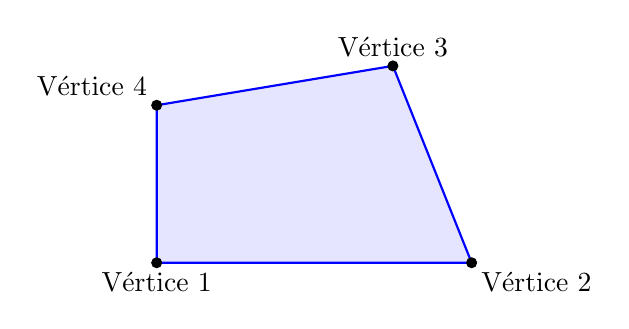
\begin{tikzpicture}
		% Desenho do polígono no plano
		\fill[blue!10] (0,0) -- (4,0) -- (3,2.5) -- (0,2) -- cycle;
		
		% Linhas (hiperplanos no plano)
		%\draw[thick, red] (0,2) -- (4,1.5) node[anchor=south east] {Hiperplano 1};
		%\draw[thick, green!70!black] (0,0) -- (4,3) node[anchor=south] {Hiperplano 2};
		%\draw[thick, purple] (0,3.5) -- (4,-0.5) node[anchor=north] {Hiperplano 3};
		
		% Polígono (interseção das restrições)
		\draw[thick, blue] (0,0) -- (4,0) -- (3,2.5) -- (0,2) -- cycle;
		
		% Vértices
		\fill[black] (0,0) circle (2pt) node[anchor=north] {Vértice 1};
		\fill[black] (4,0) circle (2pt) node[anchor=north west] {Vértice 2};
		\fill[black] (3,2.5) circle (2pt) node[anchor=south] {Vértice 3};
		\fill[black] (0,2) circle (2pt) node[anchor=south east] {Vértice 4};
		
		%Título
		%\node[below] at (2,-1) {\textbf{Figura 1: Interseção de hiperplanos em $\mathbb{R}^2$ (polígono)}};

	\end{tikzpicture}
	\caption{Interseção de hiperplanos em \(\mathbb{R}^2\)}
	\end{figure}
	
	%\vspace{2cm}
	\item No espaço tridimensional ($\mathbb{R}^3$): Um vértice de um poliedro é o ponto de encontro de três faces, que correspondem a hiperplanos em um espaço tridimensional.
	
	% Figura no espaço tridimensional (R^3)
	\begin{figure}[H]
	\centering
	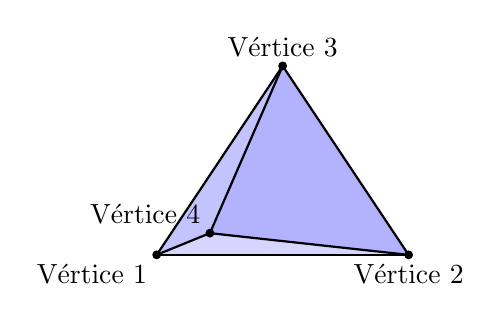
\begin{tikzpicture}[scale=0.8]
		% Poliedro (um tetraedro simples)
		\fill[blue!10,opacity=0.7] (0,0,0) -- (4,0,0) -- (2,3,0) -- cycle; % Base
		\fill[blue!20,opacity=0.7] (0,0,0) -- (4,0,0) -- (2,1.5,3) -- cycle; % Face lateral 1
		\fill[blue!30,opacity=0.7] (0,0,0) -- (2,3,0) -- (2,1.5,3) -- cycle; % Face lateral 2
		\fill[blue!40,opacity=0.7] (4,0,0) -- (2,3,0) -- (2,1.5,3) -- cycle; % Face lateral 3
		
		% Arestas do poliedro
		\draw[thick, black] (0,0,0) -- (4,0,0);
		\draw[thick, black] (4,0,0) -- (2,3,0);
		\draw[thick, black] (2,3,0) -- (0,0,0);
		\draw[thick, black] (0,0,0) -- (2,1.5,3);
		\draw[thick, black] (4,0,0) -- (2,1.5,3);
		\draw[thick, black] (2,3,0) -- (2,1.5,3);
		
		% Vértices
		\fill[black] (0,0,0) circle (2pt) node[anchor=north east] {Vértice 1};
		\fill[black] (4,0,0) circle (2pt) node[anchor=north] {Vértice 2};
		\fill[black] (2,3,0) circle (2pt) node[anchor=south] {Vértice 3};
		\fill[black] (2,1.5,3) circle (2pt) node[anchor=south east] {Vértice 4};
		
		% Título
		%\node[below] at (2,-1,0) {\textbf{Figura 2: Interseção de hiperplanos em $\mathbb{R}^3$ (poliedro)}};
	\end{tikzpicture}
	\caption{Interseção de Hiperplanos em $\mathbb{R}^3$}
	\end{figure}
\end{itemize}

Portanto, o conceito algébrico de ponto extremo está diretamente relacionado ao conceito geométrico de vértice. Concluímos que os pontos extremos de um conjunto viável de um PPL são, geometricamente, os vértices do poliedro formado por esse conjunto.
     

Pontos extremos desempenham um papel importante na Programação Linear, pois como veremos adiante, a solução ótima de um PPL sempre está em um ponto extremo do conjunto viável. Para o método simplex, a existência de pontos extremos degenerados requer precauções, pois esses podem afetar o desempenho do método, inclusive fazendo rodar indefinitivamente.   

\subsection{Raios e Direções}

Um raio também é uma classe de conjuntos convexos, que são definidos a seguir.

\begin{def:raio}
	Um raio $r$ é uma coleção de pontos dados na forma
	\begin{equation*}
		r = \{\mathbf{x} \in \mathbb{R}^n \ |\  \mathbf{x} + \lambda \mathbf{d}, \lambda > 0\}
	\end{equation*}
	onde $\mathbf{d}$ é um vetor em $\mathbb{R}^n$ não nulo e $\lambda$ é um real positivo
\end{def:raio}

Podemos também interpretar raios geometricamente como sendo uma semirreta com origem em $\mathbf{x}$, dito como o vértice do raio, e que se estende na direção do vetor $\mathbf{d}$, chamado de diretor ou direção do raio.

\begin{def:direção}
	Seja $X$ um conjunto convexo contido no $\mathbb{R}^n$. O vetor não nulo $\vec{d} \in \mathbb{R}^n$ é uma direção de $X$ com vértice em $\vec{x_0} \in X$ se para qualquer $\lambda \geq 0$ é verdade que $\vec{x_0} + \lambda \vec{d} \in X$  
\end{def:direção}

A Definição expande a noção de direção para qualquer conjunto convexo além dos raios. Dessa forma, uma direção pode ser entendida como uma semirreta que está contida num conjunto convexo. Disso segue que um conjunto convexo que possui uma direção não pode ser limitado, já que semirretas estendem-se indefinitivamente.

\begin{def:direção extrema}
	Seja $X$ um conjunto convexo e $\vec{d}$ uma direção desse conjunto. O vetor $\vec{d}$ é chamado de direção extrema se ele não pode ser dado como combinação linear positiva de outras direções desse conjunto.
\end{def:direção extrema}

A ideia de direções extremas é análoga a de pontos extremos. O vetor $\vec{d}$ é direção extrema se não existe outras duas direções $\vec{d}_1$ e $\vec{d}_2$ tal que
\begin{gather*}
	\lambda_1\vec{d}_1 + \lambda_2\vec{d}_2 = \vec{d} \\
	\lambda_1, \lambda_2 \geq 0
\end{gather*}
Os raios cuja a direção é dada por uma direção extrema são chamados de raios extremos.

Os conceitos de raios e direções podem ser usados para definir os cones convexos. Seja $C \subset \mathbb{R}^n$ um cone definido como \[C = \{\vec{x}\ |\ \lambda\vec{x}, \lambda \geq 0\}\]Podemos perceber que o subconjunto de $C$ dado pelos múltiplos escalares positivos de $\vec{x} \in C$ formam um raio com vértice na origem do $\mathbb{R}^n$ com direção dada por $\vec{x}$. Dessa forma, um cone pode ser definido a partir de suas direções, mas nem todas são necessárias para tal, já que podemos usar somente as suas direções extremas, que formam um conjunto minimal gerador das demais.

Portanto, se $C$ é um cone e $D = \{\vec{d}_1, \vec{d}_2, \ldots, \vec{d}_n\}$ o conjunto das suas direções extremas, então o cone pode ser dado como
\begin{equation*}
	C = \{\vec{x}\ |\ \vec{x} = \displaystyle\sum_{j = 1}^{n}
			\lambda_j \vec{d}_j, \lambda_j \geq 0\}
\end{equation*}

\begin{figure}[H]
\centering
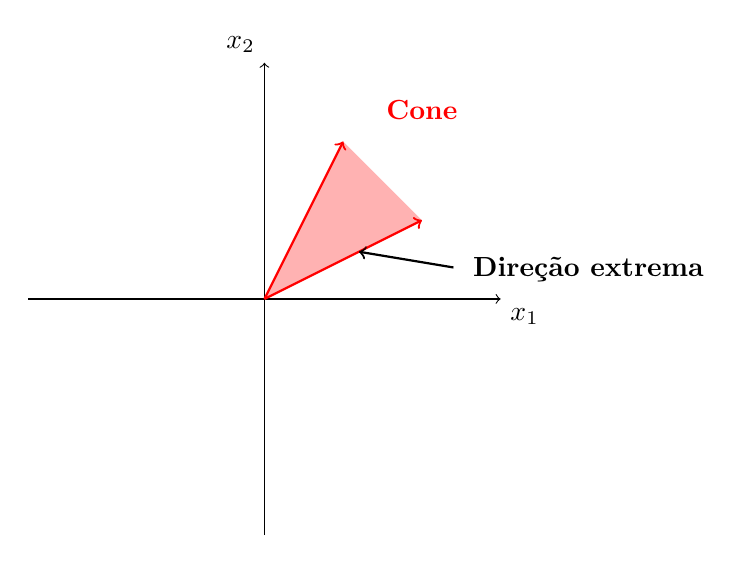
\begin{tikzpicture}[scale=2]
	
	% Eixos coordenados
	\draw[->] (-1.5, 0) -- (1.5, 0) node[below right] {\(x_1\)};
	\draw[->] (0, -1.5) -- (0, 1.5) node[above left] {\(x_2\)};
	
	% Semirretas (vetores que formam o cone)
	\draw[thick, red, ->] (0, 0) -- (1, 0.5) node[midway, above right] {};
	\draw[thick, red, ->] (0, 0) -- (0.5, 1) node[midway, above right] {};
	
	% Anotação para a direção extrema
	\draw[->, thick] (1.2, 0.2) -- (0.6, 0.3) node[pos=-0.1, right] {\textbf{Direção extrema}};
	
	
	% Região do cone (preenchida)
	\fill[red, opacity=0.3] (0, 0) -- (1, 0.5) -- (0.5, 1) -- cycle;
	
	% Vetores dentro do cone (exemplo de combinações convexas)
	%\draw[thick, blue, ->] (0, 0) -- (0.8, 0.6) node[midway, above] {};
	%\draw[thick, blue, ->] (0, 0) -- (0.4, 0.4) node[midway, above] {};
	
	% Adicionando um label para o cone
	\node[red] at (1, 1.2) {\textbf{Cone}};
\end{tikzpicture}
\caption{Representação de um Cone e seus raios extremos em \(\mathbb{R}^2\)}

\label{fig:cone}
\end{figure}

\subsection{Faces e Arestas}

Nesta seção apenas abordaremos algumas definições algébricas para conceitos historicamente geométricos. A primeira delas será a \textbf{face}.

\begin{def:face}
	Seja $X$ um conjunto convexo e $F = \{\vec{x} \in X\ |\ B\vec{x} = \vec{c}\}$ em que $B\vec{x} = \vec{c}$ é o sistema linear cujas equações é um subconjunto não vazio dos hiperplanos definidores de $X$. O conjunto $F$ é então chamado de face de $X$. 
\end{def:face}

Em outras palavras uma face é um subconjunto de $X$ cujos elementos são solução de um sistema linear dado por 1 ou mais hiperplanos de $X$. Em dimensão três, quando pensamos em faces de um poliedro, pensamos naquelas que tem dimensão dois, mas a nossa definição permite que outros elementos de dimensão menores, como as arestas e os vértices desse poliedro também sejam chamados de ``faces''. 

Na verdade, em dimensão $n$ podemos ter faces de qualquer dimensão entre 1 e $n$. As faces de dimensão $n - 1$, como as faces propriamente ditas de um poliedro em dimensão 3, ou as arestas de um polígono bidimensional, são chamadas de \textbf{facetas}. Facetas também podem ser entendidas como a parte viável (que está em $X$) de um hiperplano definidor.  As faces com dimensão entre $n - 1$ e $0$ são chamadas de faces próprias de $X$, enquanto aquela de dimensão $n$, que é o próprio $X$ é chamada de face imprópria\footnote{Se nossa definição considerasse o conjunto vazio também como face de um conjunto convexo, então ele também seria uma face imprópria}.

Vamos agora dizer que $r(F)$ da face $F$ de um conjunto convexo $X$ é o número mínimo de hiperplanos necessários para definir $F$ como o conjunto solução de um sistema linear. Esse número, para pontos extremos, que são faces de dimensão 0, é $n$, como vimos no teorema \ref{thm:ponto extremo}. Para uma aresta, que é um segmento de reta, e possui, pois, dimensão 1, esse número é $n - 1$. Podemos concluir que no geral a dimensão $\dim(F)$ de uma face $F$ e o número $r(F)$ estão relacionadas por
\begin{equation*}
	r(F)= n - \dim(F)
\end{equation*} 

Ainda sobre arestas, sabemos da geometria clássica que elas sempre conectam dois vértices, par esse chamado de adjacentes. Como vimos, pontos extremos equivalem aos vértices de um poliedro convexo $n$ dimensional, e, analogamente, os pontos extremos que são conectados por uma aresta (o que nem sempre ocorre, visto que os poliedros podem ser ilimitados) são também chamados de \textbf{adjacentes}. A Proposição a seguir mostra que dois vértices produzem uma aresta.

\begin{prop:aresta}
	O conjunto das combinações convexas de dois pontos extremos de um conjunto convexo $X$ é uma aresta de $X$
	
	\begin{proof}
		Sejam $\vec{x}_1$ e $\vec{x}_2$ pontos extremos de $X$, e digamos que $R$ e $S$ sejam os conjunto dos hiperplanos definidores de $X$ aos quais $\vec{x}_1$ e $\vec{x}_2$ pertencem respectivamente. Sob a hipótese de que $\vec{x}_1$ e $\vec{x}_2$ são distintos, então $R \cap S$ possui $n - 1$ hiperplanos, que por sua vez, devem se intersectar em uma face $E$ de dimensão $1$.
		
		Seja $C$ é o conjunto das combinações lineares convexas de $\vec{x}_1$ e $\vec{x}_2$, iremos provar que $C = E$. Primeiramente, temos que $E$ é um conjunto convexo por ser a interseção de conjuntos convexos, e como $\vec{x}_1$ e $\vec{x}_2$ pertencem a $E$, então suas combinações convexas, dadas por $C$, devem estar contidas em $E$.
		
		O próximo passo é mostrar que todos os pontos de $E$ são combinações convexas de $\vec{x}_1$ e $\vec{x}_2$, e usaremos um argumento geométrico para isso. O conjunto $E$ está numa reta, pois tem dimensão $1$, e da geometria básica sabemos que uma reta é definida por no mínimo dois pontos. Se existisse um ponto $\vec{x}_3 \in E$ que não é combinação convexa de $\vec{x}_1$ e $\vec{x}_2$, então $\vec{x}_3$ não pode estar entre $\vec{x}_1$ e $\vec{x}_2$, o que nos leva a dois casos
		\begin{itemize}
			\item $\vec{x}_1$ está entre $\vec{x}_3$ e $\vec{x}_2$
			
			\item $\vec{x}_2$ está entre $\vec{x}_1$ e $\vec{x}_3$
		\end{itemize}
		Os dois casos levam a um absurdo, pois ou $\vec{x}_1$ ou $\vec{x}_2$ estaria entre dois pontos de $E$ e não seria um ponto extremo. Concluímos então que $C = E$, e as combinações convexas de dois vértices é uma aresta. 
	\end{proof}
\end{prop:aresta}

Repare que a recíproca da proposição não é verdadeira, e um exemplo simples é o cone, como mostrado na figura \ref{fig:cone}, que possui apenas um vértice na origem, e duas arestas que se prolongam indefinitivamente. 

A ideia de adjacência entre vértices é bem simples, mas é aplicada no método simplex. Como citamos anteriormente, a busca das soluções ótimas de um PPL pelo simplex se dá nos pontos extremos da região viável, e a forma como ele realiza essas buscas é percorrendo as arestas do conjunto, ou seja, ele parte de um ponto extremo e segue a busca em um ponto extremo adjacente sempre.  


% -------------------------- DEFINIÇÃO --------------------
\newtheorem{def:convex hull}[def:conjunto convexo]{Definição}
\newtheorem{def:independencia convexa}[def:conjunto convexo]{Definição}
\newtheorem{def:simplex}[def:conjunto convexo]{Definição}
\newtheorem{def:combinação afim}[def:conjunto convexo]{Definição}

% ------------------------- PROPOSIÇÃO --------------------
\newtheorem{prop:redundancia}[prop:combinação convexa]{Proposição}
\newtheorem{prop:pontos extremos na fronteira}[prop:combinação convexa]{Proposição}
\newtheorem{prop:conjuntos convexos fechados}[prop:combinação convexa]{Proposição}
\newtheorem{prop:conjuntos convexos limitados}[prop:combinação convexa]{Proposição}

% ------------------------------ LEMA --------------------------
\newtheorem{lemma:afim}{Lema}[chapter]

%------------------------------ TEOREMA ---------------------------
\newtheorem{thm:caratheodory}{Teorema}[chapter]
\newtheorem{thm:conjuntos convexos compactos}[thm:caratheodory]{Teorema}

% ---------------------------- COROLÁRIO -----------------------
\newtheorem{cor:caratheodory}{Corolário}[chapter]

\section{Geometria dos Poliedros Convexos}

Nesta seção iremos obsevar os poliedros convexos a partir de sua
natureza geométrica ao mesmo tempo que mostramos sua equivalência com
os conceitos algébricos vistos nas seções anteriores.

\subsection{Envoltória Convexa}

\begin{def:convex hull}
	\label{def:convex hull}
	Seja $P$ um conjunto de pontos em $\mathbb{R}^n$. Chamamos de envoltória
	convexa $P$, ou fecho convexo, o conjunto
	$\conv{P}$ dado por todas as combinações convexas dos pontos de $P$
\end{def:convex hull}

Em outras referências, pode-se encontrar uma definição equivalente de que a
envoltória convexa, também popularmente conhecida como \textit{covex hull},
é o menor conjunto convexo que contém todos os pontos de $P$. Neste texto,
usaremos a definição destacada por ela ser mais algebricamente fecunda.

\begin{def:independencia convexa}
	Seja $P \subset \mathbb{R}^n$ é um conjunto de pontos. $P$ é convexo-independente
	se nenhum de seus pontos pode ser dado como combinação convexa de outros dois.
\end{def:independencia convexa}

A definição acima especializa o conceito de independência linear para conjuntos convexos,
que nos será uma definição útil. Dessa forma, um conjunto convexo-dependente será aquele
no qual há pelo menos um ponto que pode ser dado como combinação convexa de outros dois.
Outra especialização que faremos será do conceito de geradores: se um conjunto convexo
$X$ é a envoltória convexa de um conjunto $P$, então $P$ é um conjunto gerador de $X$.
Ademais, se $P$ é convexo-independente, então os pontos de $P$ são os pontos extremos
de $X$, o que especializa o conceito de base da álgebra linear para os pontos extremos.

Na Teoria de PL, nosso interesse irá se concentrar nos conjuntos convexo que são
finitamente gerados, isto é, que podem ser determinados por um conjunto finito
de pontos geradores. Exemplo de conjuntos convexos finitamente gerados são
os poliedros tridimensionais e os polígonos, enquanto que o círculo, ou a esfera,
são exemplos de conjuntos convexos que não são finitamente gerados.

\begin{figure}[h]
\centering
% Primeira figura: Polígono Convexo
\begin{subfigure}{0.45\textwidth}
	\centering
	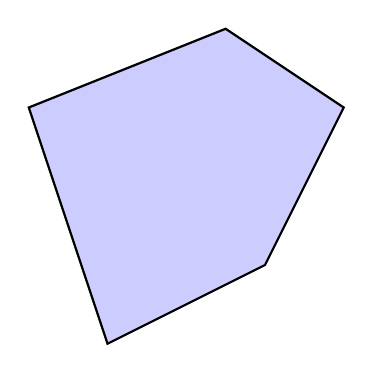
\begin{tikzpicture}
		\draw[thick, fill=blue!20] (0,0) -- (2,1) -- (3,3) -- (1.5,4) -- (-1,3) -- cycle;
	\end{tikzpicture}
	\caption{Conjunto convexo finitamente gerado}
	\label{fig:poligono}
\end{subfigure}
\hfill
% Segunda figura: Círculo
\begin{subfigure}{0.50\textwidth}
	\centering
	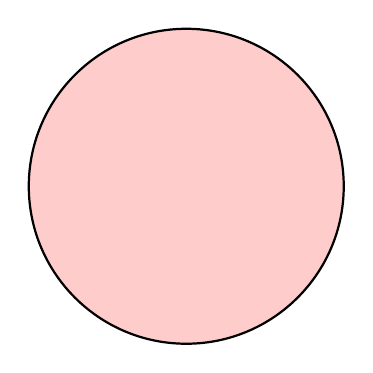
\begin{tikzpicture}
		\draw[thick, fill=red!20] (0,0) circle (2);
	\end{tikzpicture}
	\caption{Conjunto convexo não finitamente gerado}
	\label{fig:circulo}
\end{subfigure}
\caption{Comparação entre um polígono convexo e um círculo.}
\end{figure}

\begin{prop:redundancia}
	Seja $P = \{p_1, \ldots, p_m\}$ um conjunto convexo dependente e
	$P' = \{p_1, \ldots, p_k\}$ um subconjunto convexo-independente
	de $P$ com $k < m$. Então é correto dizer que
	\begin{equation*}
		\conv{P'} = \conv{P}
	\end{equation*}
\end{prop:redundancia}

Dado um conjunto de geradores, é fácil observar que, ao obtermos um
novo conjunto sem as redundâncias, então a envoltória convexa, como
foi definida em \ref{def:convex hull}, será exatamente a mesmas para
ambos os conjuntos. Além disso, se $P$ for um conjunto convexo
independente, então seus elementos são os pontos extremos de \(\conv{P}\),
como fora observado mais previamente.

Uma classe especial de envoltórias convexas são os \textbf{simplex}
A ideia geométrica por detrás do conceito de simplex é do ``mais simples
conjunto convexo num espaço euclideano de dimensão finita''. Por exemplo:
o menor número de pontos necessários para delimitar uma região no plano é
3, e a região delimitada por eles é um triângulo. Já em dimensão 3, para
delimitar uma região no espaço são necessários ao menos quatro pontos,
que definirão um tetraedro. Generalizando essa primitiva, obtemos a definição.

\begin{def:simplex}
	Chama-se simplex a envoltória convexa de um conjunto de $n+1$ pontos
	em $\mathbb{R}^n$ convexo-independente.
\end{def:simplex}

\begin{figure}[h]
	\centering
	% Primeira figura: Triângulo
	\begin{subfigure}{0.45\textwidth}
		\centering
		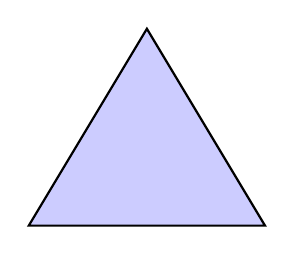
\begin{tikzpicture}
			\draw[thick, fill=blue!20] (0,0) -- (3,0) -- (1.5,2.5) -- cycle;
		\end{tikzpicture}
		\caption{Simplex em 2D}
		\label{fig:triangulo}
	\end{subfigure}
	\hfill
	% Segunda figura: Tetraedro em 3D
	\begin{subfigure}{0.45\textwidth}
		\centering
		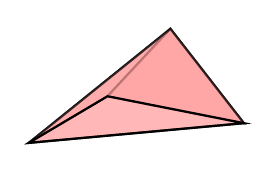
\begin{tikzpicture}
			% Definição dos vértices
			\tdplotsetmaincoords{70}{120}
			\begin{scope}[tdplot_main_coords]
				% Arestas do tetraedro
				\draw[thick, fill=red!20, opacity=0.7] (0,0,0) -- (2,0,0) -- (1,1.5,1.5) -- cycle;
				\draw[thick, fill=red!30, opacity=0.7] (0,0,0) -- (1,1.5,1.5) -- (0,2,0) -- cycle;
				\draw[thick, fill=red!40, opacity=0.7] (2,0,0) -- (1,1.5,1.5) -- (0,2,0) -- cycle;
				\draw[thick] (0,0,0) -- (2,0,0) -- (0,2,0) -- cycle;
			\end{scope}
		\end{tikzpicture}
		\caption{Simplex em 3D}
		\label{fig:tetraedro}
	\end{subfigure}
	\caption{Comparação entre simplex de dimensões diferentes.}
\end{figure}

\subsection{Espaços Afim}

Antes de ir mais afundo na natureza geométrica dos conjuntos
poliédricos, iremos recuar um pouco e observar alguns conceitos
algébricos. Relembrando, uma das noções primárias da Álgebra Linear é a de
independência linear, em que dizemos que um conjunto de vetores
é linearmente independente se nenhum vetor poder ser dado
como combinação linear dos demais. Uma classe de combinações
lineares que nos é últil são as chamadas combinações afim

\begin{def:combinação afim}
Sejam $v_1, \ldots, v_k$ vetores do $\mathbb{R}$. $u$ é uma
combinação afim dos vetores citados  se existem $\lambda_1, \ldots,
\lambda_k$ tal que
\begin{equation*}
	u = \sum_{i =1}^{k}\lambda_i v_i \quad \quad \sum_{i=1}^{k} \lambda_i = 1
\end{equation*}
\end{def:combinação afim}
Combinações afim são uma especialização das combinações
lineares, visto a restrição de que a soma dos escalares
que acompanham os vetores deve ser igual a 1. Observemos
também que as combinaçãoes convexas, por sua vez, são uma
especialização das combinações afim, em que adiciona-se a
restrição de que os pesos devem ser positivos.

As combinações lineares afim de um conjunto de vetores
formam um conjunto fechado chamado de \textbf{subsespaço afim},
que são análogos aos hiperplanos lineares a menos
da restrição de conterem a
origem do $\mathbb{R}^n$.

% imagem de compração de um hiperplano linear
% e um afim

Os hiperplanos  afins, de forma análoga ao lineares, podem ser
definidos a partir de um sistema linear na forma $Ax = b$
ou através de um conjunto de no mínimo $n$ geradores.
Um conjunto de vetores em que pelo menos um dos membros
é combinação afim dos demais é chamado de afimmente dependente.
Geometricamente, isso significa que pelo menos um dos vetores estará
no espaço afim gerado pelos demais.

É sabido que qualquer conjunto com mais de $n$ vetores em
$\mathbb{R}^n$ é linearmente dependente, mas qual será o número mínimo
de vetores em um conjunto para afirmamos com certeza que eles são
afimmente dependentes?

A envoltória convexa de dois pontos é um segmento de reta, e,
por sua vez, o subsespaço afim gerado por esses mesmos pontos é a
a própria reta que eles definem, ou seja, obtemos o subespaço
afim gerado ao extender infinitamente o segmento de reta em
ambos os seus sentido. Já três pontos não colineares
definem um triângulo, que é uma figura plana, e o subsespaço afim gerado por
esses três pontos é justamnte o plano que contém esse triângulo; é como se
tivessemos expandido infinitamente a área do triângulo assim como fizemos
com o comprimento do segmento de reta anteriormente. Por conseguinte,
para obter o \textit{span} afim a partir de uma envoltória convexa, basta
extendemos infinitamente a envoltória nas direções possíveis.

Isso nos permite agora responder a questão feita mais atrás:
expandir infinitamente um simplex de dimensão $n$ que é gerado
por $n+1$ vetores do  $\mathbb{R}^n$,
, é suficiente para obtermos todo o $\mathbb{R}^n$
e qualquer outro vetor do $\mathbb{R}^n$ pode ser dado como
combinação afim dos pontos extremos do simplex que fora expandido.
Portanto, a conclusão que chegamos é que qualquer conjunto com mais
de $n+1$ vetores é necessariamnte afimmente independente. Esse resultado
é provado formalmente com uma abordagem mais algébrica no lema a seguir.

\begin{lemma:afim}
	\label{lemma:afim}
	Se $P = \{p_1, \ldots, p_k\} \subset \mathbb{R}^n$ é um conjunto
	finito de pontos com $k > n + 1$, então existem $\mu_1, \ldots, \mu_n
	\in \mathbb{R}$ não todos nulos tal que
	\begin{equation*}
		\displaystyle\sum_{i=1}^k \mu_i p_i = 0 \quad\quad \displaystyle\sum_{i=1}^k \mu_i = 0
	\end{equation*}
	e $P$ é um conjunto afimmente dependente.

	\begin{proof}
		Da álgebra linear, sabemos que, se $\#P = k > n$, então $P$ é um conjunto
		linearmente dependente, o que implica dizer que há $\mu_1, \ldots, \mu_n
		\in \mathbb{R}$ não todos nulos tal que
		\[\displaystyle\sum_{i=1}^k \mu_i p_i = 0\]

		Além disso, observemos que o conjunto $\{p_2 - p_1, \ldots, p_k - p_1\}$
		também é linearmente dependente, portanto
		\[\displaystyle\sum_{i=2}^k \mu_i (p_i - p_1) = 0\]
		e fazendo \(\mu_1 = -\displaystyle\sum_{i=2}^k \mu_i\)
		obtemos que
		\[\displaystyle\sum_{i=1}^k \mu_i = 0\]

		Resta mostrar que o conjunto $P$ é afimmente dependente. Para isso, suponha
		que $P$ esteja ordenado de forma que para todo $i \in I = \{1, \ldots, n\}$
		é verdade que $\mu_k \geq \mu_i$. Obeservamos então que
	  \begin{gather*}
	    \mu_1 p_1 + \ldots + \mu_{k - 1} p_{k-1} + \mu_k p_k = 0 \\
      \mu_1 p_1 + \ldots + \mu_{k - 1} p_{k-1} = - \mu_k p_k \\
	  \end{gather*}
	  Dividindo a equação acima toda por $-\mu_k$ otbemos
	  \begin{gather*}
	    \sum_{i=1}^{k-1} -\frac{\mu_i}{\mu_k} p_i = p_k
	  \end{gather*}
	  Mas também
	  \begin{gather*}
      \sum_{i=1}^{k-1} \mu_i = 0 \\
	    \sum_{i=1}^{k-1} -\frac{\mu_i}{\mu_k} = 1
	  \end{gather*}
	  Portanto $p_k$ pode ser dado como combinação afim dos demais pontos de
	  $P$, e o conjunto dos pontos é afimmente dependente.
	\end{proof}
\end{lemma:afim}

\subsection{Teorema de Carathéodory}

O Teorema de Carathéodory é um dos resultados mais fundamentais da geometria
convexa, pois ele nos permite dizer que um ponto qualquer em um conjunto
convexo pode ser gerado por um número finito de outros pontos nesse conjunto,
mas não somente isso como também o limitante do tamanho desse conjunto de
geradores.

\begin{thm:caratheodory}[Carathéodory]
	Seja $P \subset \mathbb{R}^n$ um conjunto finito de pontos. Se $x \in \conv{P}$, então
	$x \in \conv{P'}$ para algum $P' \subset P$ com cardinalidade igual a $n + 1$.

	\begin{proof}
		Com efeito, se $x \in \conv{P}$, e $\#P = k$, então existem $\lambda_1, \ldots, \lambda_k
		\in \mathbb{R}$ com $\lambda_i \in [0, 1]$ tal que
		\begin{equation}
		\label{eq_thm_caratheory}
		\begin{gathered}
			x = \displaystyle\sum_{i=1}^k \lambda_i p_i \\
			\displaystyle\sum_{i=1}^k \mu_i = 1
		\end{gathered}
		\end{equation}
		Se $k \leq n + 1$, então nada há a demonstrar, do contrário, o lema \ref{lemma:afim}
		garante que existem $\mu_1, \ldots, \mu_n \in \mathbb{R}$ não todos nulos tal que
		\[\displaystyle\sum_{i=1}^k \mu_i p_i = 0\]
		e como \(\alpha \displaystyle\sum_{i=1}^k \mu_i p_i = 0\) para todo $\alpha \in \mathbb{R}$
		então podemos rescrever a equação \ref{eq_thm_caratheory} como
		\begin{gather*}
			x = \displaystyle\sum_{i=1}^k \lambda_i p_i - \alpha \displaystyle\sum_{i=1}^k \mu_i p_i \\
			x = \displaystyle\sum_{i=1}^k (\lambda_i - \alpha \mu_i) p_i
		\end{gather*}
		donde temos que
		\[\displaystyle\sum_{i=1}^k (\lambda_i - \alpha \mu_i) = 1\]

		Agora iremos tentar escrever $x$ como uma combinação convexa de até $n + 1$ pontos.
		Para atingir esse objetivo, escolhemos $\alpha$ tal que
	\[\alpha  = \min{\frac{\lambda_i}{\mu_i}\  |\  i \in \{1,\ldots, k\} \text{ e } \mu_i > 0}\]
		Logo, $\alpha > 0$, e para $i \in \{1, \ldots, k\}$, temos dois casos.

		I - $\mu_i \geq 0$

		Temos que
		\[\lambda_i - \alpha \mu_i = \mu_i \left(\frac{\lambda_i}{\mu_i} - \alpha\right)\]
		e pela nossa escolha de $\alpha$, então \(\lambda_i - \alpha \mu_i \geq 0\)

		II - $\mu_i < 0$

		Uma vez que $\alpha > 0$, então $\alpha \mu_i > 0$ e, portanto,
		\(\lambda_i - \alpha \mu_i \geq 0\)

		digamos que $j*$ seja tal que $\alpha = \frac{\lambda_{j^*}}{\mu_{j^*}}$. Observe que
		$\lambda_{j^*} - \alpha \mu_{j^*}$, e podemos expressar $x$ como
		\[x = \displaystyle\sum_{i=1}^{j^* - 1} (\lambda_i - \alpha \mu_i)p_i +
				\displaystyle\sum_{i=j^* + 1}^{k} (\lambda_i - \alpha \mu_i)p_i\]
		donde concluímos que $x$ pode ser escrito como combinação convexa de $k - 1$ pontos de $conv{P}$

		Como podemos repetir esse processo enquanto $k > n + 1$, ou seja, enquanto o lema \ref{lemma:afim}
		pode ser aplicado, então $x$ pode ser escrito como combinação convexa de até $n + 1$ pontos de $\conv{P}$.
	\end{proof}
\end{thm:caratheodory}

Para capturar o significado geométrico do Teorema de Carathéodory, poderíamos
enunciá-lo como ``um ponto qualquer num fecho convexo sempre estará no interior
de um simplex gerado por pontos desse fecho''. Ademais, se $P \subset \mathbb{R}^n$ é um conjunto
convexo-independente, então para qualquer $x \in \conv{P}$, $x$ pode ser dado
como combinação convexa de até $n+1$ pontos de $P$, ou seja, de até $n+1$ pontos extremos.
Formalizemos essa conclusão como corolário do Teorema de Carathéodory.

\begin{cor:caratheodory}
	Seja $P \subset \mathbb{R}^n$ um conjunto convexo-independente. Se $x \in \conv{P}$
	então $x$ pode ser dado como combinação convexa de até $n + 1$ pontos de $P$
\end{cor:caratheodory}

Em outras palavras, o corolário afirma que um ponto qualquer num fecho convexo
pode ser dado como combinação convexa de até $n+1$ pontos extremos.

\subsection{Topologia de Evoltórias Convexas}

Nesta seção iremos analisar algumas propriedades topológicas básicas de
interesse sobre a envoltória convexa de um conjunto de pontos. Mas não se
preocupe, apesar de usarmos conceitos de topologia, iremos apresentá-los
e usá-los de forma bem elementar a fim de não desviar muito dos nossos
objetios e complicar em demasiado nossas construções, já que está fora do
escopo desse texto as noções mais aprofundadas desse tema.

\begin{prop:pontos extremos na fronteira}
Seja $P$ um conjunto convexo. Se $\bar{\vec{x}}$ é um ponto extremo de $P$,
então $\bar{\vec{x}}$ é um ponto na fronteira de $P$.

  \begin{proof}
    Para provarmos esse resultado, basta mostrarmos que para qualquer bola
    aberta $B$ centrada em $\bar{\vec{x}}$, $B$ intercepta pontos tanto de
    $P$ quanto de $\mathbb{R}^n / P$. Suponha por contradição que haja uma
    bola aberta centrada em $\bar{\vec{x}}$ tal que $B \subsetneq P$. Isso
    implica que $\bar{\vec{x}}$ está no interior de um segmento de reta
    inteiramente contido em $P$, e não é, pois, ponto extremo.
  \end{proof}
\end{prop:pontos extremos na fronteira}

\begin{prop:conjuntos convexos fechados}
Se $C$ é a envoltória convexa de $P$, então $C$ é fechado.

  \begin{proof}
   Seja $\vec{x}$ um ponto na fronteira $F$ de $C$. É trivial o fato de que se
   $\vec{x}$ é um ponto extremo de $C$, então $\vec{x} \in P$. Se
   $\vec{x} \in F$ não for um ponto extremo, então uma vez que $\vec{x} \in F$,
   temos que existe uma vizinhança $V$ de $\vec{x}$ que contém um ponto $\vec{y}$
   tal que $\vec{y} \in C$.

   Digamos que $\vec{d} = \vec{x} - \vec{y}$, e todo ponto dado como \[
     \vec{y} + (1 - \epsilon) \vec{d}
   \]com $\epsilon \in (0, 1]$ faz parte de um raio contido em $C$. Repare que
   esse ponto é $x$ quando $\epsilon = 0$. Digamos também que \[
     \vec{y} = \sum_{i=1}^{k} \lambda_i \vec{p_i}, \quad \vec{p_i}  \in P
   \]Das equações dadas até então, temos que
   \begin{align*}
     \vec{y} + (1 - \epsilon) (\vec{x} - \vec{y}) &= (1 + \epsilon) \vec{x}
     + \epsilon y \\
                                                  &= (1 - \epsilon) \vec{x} + \epsilon \vec{y}
   \end{align*}
   Reparemos que como estamos considerando os pontos do raio que estão no
   interior de $C$, então esses pontos
   admitem uma representação como uma combinação linear convexa dos pontos de
   $P$, ou seja
   \[
     \forall \epsilon \in (0, 1] , \exists \mu_1, \dots, \mu_k \in \mathbb{R},
     (1-\epsilon)\vec{x} + \epsilon \vec{y} = \sum_{i=1}^{k} \mu_i p_i
   \]
   Isolando $\vec{x}$ na equação acima, e adotando a representação de $\vec{y}$
   como combinação convexa, obtemos que

   \begin{equation}
     \label{eq:conjunto convexos fechados}
     \vec{x} = \sum_{i=1}^{k} \frac{(\mu_i  - \epsilon \lambda)}{1-\epsilon} \vec{p_i}
   \end{equation}
   Percebamos que
   \[
    \sum_{i=1}^{k} \frac{(\mu_i  - \epsilon \lambda)}{1-\epsilon} =
    \frac{1}{1-\epsilon}\left(
      \sum_{i=1}^{k} \mu_i -   \epsilon \sum_{i=1}^{k} \lambda_i\right)
   \]
   Uma vez que
   \[
    \sum_{i=1}^{k} \mu_i = 1 \quad \sum_{i=1}^{k} \lambda_i = 1
   \]
   obtém-se que
   \[
   \sum_{i=1}^{k} \frac{(\mu_i  - \epsilon \lambda)}{1-\epsilon} =
   \frac{1}{1-\epsilon} \cdot (1 - \epsilon) = 1
   \]
   o que vale para todo $\epsilon \in [0, 1]$.

   Se fazemos $\epsilon$ pequeno o suficiente, então a equação
   \ref{eq:conjunto convexos fechados} expressa $\vec{x}$ como combinação
   convexa de pontos de $P$
   \[
     \lim_{\epsilon \to 0} \sum_{i=1}^{k} \frac{(\mu_i  - \epsilon \lambda)}{1-\epsilon} \vec{p}_i
     = \sum_{i=1}^{k} \mu_i \vec{p}_i
   \]
   Portanto, se $\vec{x}$ está na fronteira de $C = \conv{P}$, então
   $\vec{x} \in C$.
 \end{proof}
\end{prop:conjuntos convexos fechados}

\begin{prop:conjuntos convexos limitados}
  Se $C = \conv{P}$ é a envoltória convexa de um conjunto finito $P$ de pontos,
  então $C$ é limitado.

  \begin{proof}
   Com efeito, uma vez que $P$ é finito, então deve have uma bola aberta que
   contém todos os seus pontos e, por conseguinte, a envoltória convexa desse
   conjunto, portanto $C = \conv{P}$ é limitado.
  \end{proof}
\end{prop:conjuntos convexos limitados}

Para fins de síntese, reunamos as proposiçõe anteriores no teorema a seguir

\begin{thm:conjuntos convexos compactos}
  Se $C = \conv{P}$ é a envoltória convexa de um conjunto finito de pontos,
  então $C$ é compacto.\footnote{Chama-se de compactos os conjuntos que são
  simultâneamente fechados e limitados.}
\end{thm:conjuntos convexos compactos}


\chapter{Método Simplex}

\chapter{Solução Inicial e Convergência}

\chapter{Dualidade}

\chapter{Programação Linear Inteira}


\end{document}